\chapter{NMR theory}
\label{chpt:theory}

% \epigraph{\singlespacing%
% And remember that, if you are ever so forward and clever yourselves, you should always be modest; for, much as you know already, there is a great deal more for you to learn.
% }{--- \textsc{Jane Austen}, \textit{Mansfield Park}}

\epigraph{\singlespacing%
I have seen a great many lists of her drawing-up at various times of books that she meant to read regularly through—and very good lists they were---very well chosen, and very neatly arranged \ldots{} But I have done with expecting any course of steady reading from Emma. She will never submit to any thing requiring industry and patience.
}{--- \textsc{Jane Austen}, \textit{Emma}}

In the opening chapter of this thesis, I provide an overview of basic NMR theory, specifically, the dynamics of quantum systems containing one or more spin-\half{} particles.
Starting from the Schr\"odinger equation, I progressively develop the rotating frame and density operator formalisms used in the analysis and simulation of simple NMR experiments.
The important product operator formalism, used throughout this thesis, is exemplified through a selection of 1D and 2D experiments.
Since 2D experiments form a very large part of this thesis, I also discuss a number of general principles in 2D NMR.

Note that this chapter is not intended to be an exhaustive account of magnetic resonance theory; for more complete coverage, the reader is directed to a suitable textbook\autociteset{textbooks-theory}.

\clearpage

\section{Quantum mechanics}
\label{sec:theory__quantum_mechanics}

The most fundamental equation in (non-relativistic) quantum mechanics, which governs the time evolution of a quantum state $\ket{\Psi(t)}$ under a Hamiltonian $H$, is the time-dependent Schr\"{o}dinger equation:
\begin{equation}
    \label{eq:tdse}
    \frac{\partial\ket{\Psi(t)}}{\partial t} = -\frac{\mi}{\hbar}H\ket{\Psi(t)} 
\end{equation}
For a Hamiltonian which is constant over a period of time $t_1 \leq t \leq t_2$ (i.e.\ is \textit{time-independent}), this can be integrated to yield an explicit solution:
\begin{equation}
    \label{eq:time_evolution}
    \ket{\Psi(t_2)} = \exp\left[-\frac{\mi H (t_2 - t_1)}{\hbar}\right]\ket{\Psi(t_1)}
\end{equation}
In NMR, it is conventional to use units of angular frequencies instead of energies, for example by replacing $H/\hbar \to H$; this will henceforth be assumed.
The term $\exp[-\mi H(t_2 - t_1)]$ is called the \textit{propagator} of the system and denoted $U(t_2, t_1)$; this is often further simplified to $U(\tau)$ where $\tau = t_2 - t_1$ is the duration of the evolution.
For a Hamiltonian which varies with time but is piecewise constant, in that it can be broken up into several finite periods within which $H\/$ is time-independent, the time evolution of the state is simply given by successive application of propagators:
\begin{equation}
    \label{eq:time_evolution_piecewise}
    \ket{\Psi(t_n)} = U(t_n,t_{n-1})\cdots U(t_2,t_1)U(t_1,t_0) \ket{\Psi(t_0)}
\end{equation}
where $t_n > t_{n-1} > \cdots > t_0$.
The case where $H\/$ continuously varies with time is more complicated, but we will not need to consider it in this thesis.

In NMR spectroscopy, we manipulate the \textit{spin angular momentum} of atomic nuclei in order to obtain information about chemical structure and dynamics.
The present work is restricted to nuclei with spin quantum number $I = 1/2$.
These are two-level systems, where the eigenstates of $I_z$ (denoted as $\ket{\alpha}$ and $\ket{\beta}$ for $m_I = +1/2$ and $-1/2$ respectively) are used as a standard basis, called the \textit{Zeeman basis}.
The $z$-axis is conventionally chosen as the quantisation axis in textbook treatments of angular momentum (primarily for mathematical convenience), but in the context of NMR, it bears even more significance as we define the $z$-axis to be the axis along which the static magnetic field is aligned.
Since the matrix elements of an operator $O$ are given by $O_{mn} = \braket{m|O|n}$, we can work out the matrix representations of the angular momentum operators in the Zeeman basis:
\begin{equation}
    \label{eq:pauli}
    I_x = \frac{1}{2}\begin{pmatrix} 0 & 1 \\ 1 & 0 \end{pmatrix}; \quad 
    I_y = \frac{1}{2}\begin{pmatrix} 0 & -\mi \\ \mi & 0 \end{pmatrix}; \quad 
    I_z = \frac{1}{2}\begin{pmatrix} 1 & 0 \\ 0 & -1 \end{pmatrix}
\end{equation}
Their commutators are given by:
\begin{equation}
    \label{eq:angmom_commutators}
    [I_i, I_j] = \sum_{k} \mi \varepsilon_{ijk}J_k,
\end{equation}
where $\varepsilon_{ijk}$ is the Levi-Civita symbol.
We also define the following linear combinations:
\begin{equation}
    % see https://stackoverflow.com/a/2600374/7115316 for equation label alignment
    \label{eq:other_single_spin_ops}
    \begin{aligned}
        I_+ = I_x + \mi I_y &= \begin{pmatrix} 0 & 1 \\ 0 & 0 \end{pmatrix}; &
        I_\alpha = \frac{1}{2}E + I_z &= \begin{pmatrix} 1 & 0 \\ 0 & 0 \end{pmatrix} \\
        I_- = I_x - \mi I_y &= \begin{pmatrix} 0 & 0 \\ 1 & 0 \end{pmatrix}; &
        I_\beta = \frac{1}{2}E - I_z &= \begin{pmatrix} 0 & 0 \\ 0 & 1 \end{pmatrix}
    \end{aligned}
\end{equation}
where $E\/$ is the $2 \times 2$ identity matrix.
The \textit{coherence order} of an operator, denoted $p$, is defined by the Zeeman basis states it connects, i.e.\ the nonzero elements in its matrix form when expressed in this basis: an operator $O = \ket{m_2}\bra{m_1}$ would represent $(m_2 - m_1)$-order coherence, since $\braket{m_2|O|m_1} \neq 0$.
Thus, in the above equations, $I_+ = \ket{\alpha}\bra{\beta}$ represents a coherence order of $+1$; $I_-$ a coherence order of $-1$; $I_x$ and $I_y$ are both a mixture of $\pm 1$-coherence; and the remainder have coherence order $0$.

States (and operators) for composite systems are formally defined as tensor products of single-spin states (and operators)\autocite{Sakurai2021}.
Operators on the same spin commute as per \cref{eq:angmom_commutators}, and operators on different spins fully commute.
The Kronecker product allows these operators to be expressed in matrix form.\autocite{Hore2015}
For example, the operator $2I_xS_z$ can be represented as follows:\footnote{This representation is not unique; it is perfectly possible to reverse the order of the Kronecker product, and as long as this is consistently done, any physically measurable quantities calculated using this alternative will be the same.}
\begin{equation}
    \label{eq:composite_operator}
    2I_xS_z = 2 \cdot \frac{1}{2} \cdot \frac{1}{2} \left[ 
    \begin{pmatrix} 0 & 1 \\ 1 & 0 \end{pmatrix} \otimes
    \begin{pmatrix} 1 & 0 \\ 0 & -1 \end{pmatrix} \right]
    = \frac{1}{2} \begin{pmatrix} 0 & 0 & 1 & 0 \\ 0 & 0 & 0 & -1 \\ 1 & 0 & 0 & 0 \\ 0 & -1 & 0 & 0 \end{pmatrix}
\end{equation}
The Hamiltonians $H\/$ for nuclear spin interactions, which will be encountered frequently in this chapter, are formed from such operators.\autocite{Levitt2008}
In solution-state NMR, these interactions include:
\begin{align}
    H_\text{cs} &= \sum_i \omega_{0,i} I_{iz} & &\text{(chemical shift)} \label{eq:h_cs} \\
    H_\text{J} &= \sum_{i > j} 2\pi J_{ij} \,(\symbf{I}_{i}\cdot \symbf{I}_{j}) & &\text{(scalar coupling)} \label{eq:h_j} \\
    H_\text{pulse} &= \sum_i \omega_{i,x}I_{ix} + \sum_i \omega_{i,y}I_{iy} & &\text{(radiofrequency pulses)} \label{eq:h_pulse} \\
    H_\text{grad} &= \sum_i \gamma_i Gz I_{iz} & &\text{(pulsed field gradients on }z\text{)} \label{eq:h_grad}
\end{align}
Pulsed field gradients (henceforth shortened to \textit{gradients}) can in principle be applied along any axis, not just $z$, but this is dependent on hardware: all the work in this thesis was done on $z$-gradient probes.
In the above expressions:

\begin{itemize}
    \item $\gamma_i$ is the magnetogyric ratio of spin $i$;
    \item $\omega_{0,i}$ refers to the Larmor, or precession, frequency of spin $i$ (usually on the order of \unit{MHz}). The Larmor frequency is defined as
        \begin{equation}
            \label{eq:larmor_frequency}
            \omega_{0,i} = -\gamma_i B_0,
        \end{equation}
        where $B_0$ is the strength of the external (static) magnetic field;
    \item $J_{ij}$ is the scalar coupling constant between spins $i$ and $j$ (expressed in units of \unit{Hz});
    \item $\omega_x$ and $\omega_y$ are amplitudes of radiofrequency (RF) pulses along the $x$- and $y$-axes, which are in general time-dependent, and are related to the so-called $B_1$ by a factor of $\gamma_i$.
    \item $G$ is the amplitude of the gradient, typically in units of \unit{G\per\cm}; and
    \item $z$ is the position of the spin along the $z$-axis, typically in units of \unit{\cm}.
\end{itemize}

Finally, note that in the \textit{weak coupling} regime where
\begin{equation}
    \omega_{0,i} - \omega_{0,j} \gg J_{ij}, \label{eq:weak_coupling}
\end{equation}
the scalar coupling Hamiltonian may be simplified (the \textit{secular approximation}\footnote{This result comes from the use of time-independent nondegenerate perturbation theory: it is based on the assumption that the eigenstates $\{\ket{n}\}$ of the main Hamiltonian $H_0$ are unchanged by the perturbation $V$ (since the first-order correction varies as $\sum_m V_{mn}/(\omega_m - \omega_n) \ll 1$), and only the first-order correction to the energies $E_n^{(1)} = \braket{n | V | n}$ is retained. In this context, $H_0$ and $V$ are respectively $H_\text{cs}$ and $H_\text{J}$. When the condition \cref{eq:weak_coupling} does not hold, the nondegenerate treatment fails; see e.g.\ Sakurai\autocite{Sakurai2021}.}) to
\begin{equation}
    H_\text{J,secular} = \sum_{i > j} 2\pi J_{ij} I_{iz}I_{jz} \label{eq:h_j_secular}.
\end{equation}
This condition is always satisfied whenever spins $i$ and $j$ are different nuclides.

Throughout the course of an NMR experiment, RF pulses and gradients are turned on and off, and thus $H_\text{pulse}$ and $H_\text{grad}$ are time-dependent---although they will always satisfy the `piecewise constant' criterion which allows us to use \cref{eq:time_evolution_piecewise}.
The `free precession' (or simply `free') Hamiltonian, $H_\text{free}$, refers to the Hamiltonian which is operative whenever no pulses or gradients are being applied: 
\begin{equation}
    \label{eq:h_free}
    H_\text{free} = H_\text{cs} + H_\text{J}.
\end{equation}


\section{The rotating frame}
\label{sec:theory__rotating_frame}

The Hamiltonians described above refer to the `laboratory frame' or the \textit{Schr\"odinger picture}, where spins precess about the $z$-axis at their intrinsic frequencies and obey the equation of motion \labelcref{eq:tdse}.
However, this proves to often be unwieldy, in particular when analysing the effects of RF pulses.
It is standard procedure to transform the frame of reference to a `rotating frame', specifically, one which rotates about the $z$-axis at a defined rotation frequency $\omegarot$ which is close to the Larmor frequencies $\omega_0$.

The rotating frame can be formalised using the \textit{interaction picture} of quantum mechanics,\autocite{Sakurai2021} which involves the separation of the Hamiltonian into two parts, with the first typically being completely time-independent:
\begin{equation}
    \label{eq:interaction_ham}
    H(t) = H_0 + H_1(t).
\end{equation}
In this case, the static part $H_0$ simply corresponds to precession of the spins at a particular frequency:
\begin{equation}
    \label{eq:interaction_ham0}
    H_0 = \sum_i \omega_{\text{rot},i}I_{iz}.
\end{equation}
(Generally, each instance of the same nuclide (e.g.\ \proton{} or \carbon{}) will share the same $\omegarot$, so the subscript $i$ in $\omega_{\text{rot},i}$ is useful only for distinguishing different nuclear species.)
This allows us to define $H_1$ as
\begin{align}
    \label{eq:reduced_ham}
    H_1 &= H_\text{J} + H_\text{pulse} + H_\text{grad} + \left(H_\text{cs} - H_0\right) \\[7pt] \notag
        &= H_\text{J} + H_\text{pulse} + H_\text{grad} + \sum_i \Omega_i I_{iz} \\ \notag
        &= H_\text{J} + H_\text{pulse} + H_\text{grad} + H_\text{offset}
\end{align}
where $\Omega_i = \omega_{0,i} - \omega_{\text{rot},i}$ is the \textit{offset} of spin $i$.
For reasons which will become clear later, the frequency $\omegarot$ is chosen to be the centre of the spectral window for the given nuclide.

Having split up our Hamiltonian, we then define an \textit{interaction-picture ket}:
\begin{equation}
    \label{eq:interaction_state}
    \ket{\Psi}_I = \exp(\mi H_0 t)\ket{\Psi}.
\end{equation}
The time evolution of this ket is given by a transformation of the Schr\"odinger equation:
\begin{align}
    \label{eq:interaction_evolution}
    \frac{\partial\ket{\Psi}_I}{\partial t} &= \mi H_0 \exp(\mi H_0 t) \ket{\Psi} + \exp(\mi H_0 t)\frac{\partial \ket{\Psi}}{\partial t} \notag \\
                                            &= \mi H_0 \ket{\Psi}_I + \exp(\mi H_0 t) (-\mi H\ket{\Psi}) \notag \\
                                            &= \mi H_0 \ket{\Psi}_I - \mi\exp(\mi H_0t)(H_0 + H_1)\exp(-\mi H_0 t)\ket{\Psi}_I \notag \\
                                            &= \mi H_0 \ket{\Psi}_I - \mi H_0\ket{\Psi}_I - \mi\exp(\mi H_0t)H_1\!\exp(-\mi H_0 t)\ket{\Psi}_I \notag \\
                                            &= -\mi\exp(\mi H_0 t)H_1\!\exp(-\mi H_0 t)\ket{\Psi}_I \notag \\
                                            &= -\mi H_{1,I}\ket{\Psi}_I,
\end{align}
where
\begin{equation}
    \label{eq:interaction_h1i}
    H_{1,I} = \exp(\mi H_0 t) H_1 \!\exp(-\mi H_0 t).
\end{equation}
The underlying principle here is that the `interesting' behaviour should be contained in $H_1$, and instead of explicitly considering the time evolution under the `uninteresting' $H_0$, it is just used to transform $H_1$ into $H_{1,I}$.

We now turn our attention to how the various NMR Hamiltonians (\cref{eq:h_cs,eq:h_j,eq:h_pulse,eq:h_grad}) are transformed in the interaction picture; that is to say, what the individual terms in the right-hand side of
\begin{equation}
    \label{eq:interaction_nmr_hamiltonians}
    \begin{aligned}
        H_{1,I} &= \exp(\mi H_0 t) H_\text{J} \exp(-\mi H_0 t) + \exp(\mi H_0 t) H_\text{pulse} \exp(-\mi H_0 t) \\
                &\quad + \exp(\mi H_0 t) H_\text{grad} \exp(-\mi H_0 t) + \exp(\mi H_0 t) H_\text{offset} \exp(-\mi H_0 t)
    \end{aligned}
\end{equation}
are.
We first note that $H_0$ (and hence $\exp(\pm \mi H_0t)$) is a function only of the $I_{iz}$ operators; thus, any Hamiltonian which commutes with all $I_{iz}$'s will be untouched by this transformation.
This is trivially true of $H_\text{offset}$ and $H_\text{grad}$, which are themselves both functions of the $I_{iz}$'s.
It can also be shown that $H_\text{J}$ (in the homonuclear case) and $H_\text{J,secular}$ (heteronuclear case) fully commute with $H_0$.
So, for three of the four terms in \cref{eq:interaction_nmr_hamiltonians} we simply have the result that $\exp(\mi H_0t)H\exp(-\mi H_0t) = H$.
This allows us to immediately write down the free precession Hamiltonian in the interaction picture:
\begin{equation}
    \label{eq:h_free_interaction}
    H_{\text{free},I} = H_\text{offset} + H_\text{J}.
\end{equation}
The fourth term, which does not commute with $H_0$, is $H_\text{pulse}$.
In the laboratory frame, \textit{hard pulses} are applied as oscillating RF fields.
Consider the case of a pulse acting on a single spin:
\begin{equation}
    \label{eq:hard_pulse}
    H_\text{pulse,hard} = \omega_1 [\cos(\omegarf t + \phi) I_x + \sin(\omegarf t + \phi) I_y].
\end{equation}
Here, $\omega_1$ represents the \textit{amplitude} of the pulse, and $\phi$ the \textit{phase}. This expression is similar to the expression in \cref{eq:h_pulse}, but here $\omega_1$ and $\phi$ are both constants, with the time dependence explicitly specified using the \textit{frequency} of the pulse, $\omegarf$.
In the rotating frame, using that $H_0 = \omegarot I_z$, we then have the following interaction Hamiltonian:
\begin{equation}
    \label{eq:hard_pulse_rotatingframe_intermediate}
    \begin{aligned}
        H_{\text{pulse,hard,}I} &= \omega_1 \,\big[\! \exp(\mi \omegarot t I_z) I_x \cos(\omegarf t + \phi) \exp(-\mi \omegarot t I_z) \\
                                &\quad\quad\quad + \exp(\mi \omegarot t I_z) I_y \sin(\omegarf t + \phi) \exp(-\mi \omegarot t I_z) \big],
    \end{aligned}
\end{equation}
and using the formulae
\begin{align}
    \exp(\mi\theta I_z)I_x\exp(-\mi\theta I_z) = I_x\cos\theta - I_y\sin\theta \label{eq:sandwich_formula_1} \\
    \exp(\mi\theta I_z)I_y\exp(-\mi\theta I_z) = I_y\cos\theta + I_x\sin\theta \label{eq:sandwich_formula_2}
\end{align}
(see Appendix A.2 of Levitt\autocite{Levitt2008} for a derivation), \cref{eq:hard_pulse_rotatingframe_intermediate} simplifies to
\begin{equation}
    \label{eq:hard_pulse_rotatingframe}
    H_{\text{pulse,hard,}I} = \omega_1 \left[I_x \cos(\omegarf - \omegarot + \phi) + I_y \sin(\omegarf - \omegarot + \phi) \right].
\end{equation}
The frequency at which hard pulses are applied is termed the \textit{transmitter frequency}, $\omegatx$.
This is a parameter which can be controlled by the user, and is typically placed in the centre of the spectrum of the sample under study, in order to make the most use of its \textit{bandwidth} (the region of frequencies over which the pulse is effective).
For convenience, it is typical to then choose the rotating-frame frequency to be exactly the same frequency: $\omegarot = \omegatx$.
This allows us to simplify the rotating-frame Hamiltonian to
\begin{equation}
    \label{eq:hard_pulse_onresonance}
    H_{\text{pulse,hard,}I} = \omega_1 (I_x\cos\phi + I_y\sin\phi),
\end{equation}
which is time-\textit{independent}.
Occasionally, I will also use the Cartesian components:
\begin{equation}
    \label{eq:pulse_cartesian}
    (c_x, c_y) = (\omega_1 \cos\phi, \omega_1 \sin\phi),
\end{equation}
instead of the amplitude and phase, to describe the pulse.

Consider now the application of this pulse to an isolated spin for which $\omega_0 = \omegarot$ and thus has an offset $\Omega = 0$.
We have that $H_\text{offset} = H_\text{J} = H_\text{grad} = 0$, and the only active Hamiltonian is that of the pulse, which causes \textit{nutation} of the spin magnetisation vector around the axis of the pulse; in this case, the pulse (or the spin) is said to be \textit{on-resonance}.%
\footnote{Strictly speaking, the rotating frame is just a mathematical formalism, so the resonance condition does not necessitate $\Omega = 0$ or $\omegarf = \omegarot = \omega_0$. We only need that $\omegarf = \omega_0$, or in other words, that the pulse is applied at the frequency of the spin---which may or may not be the same as the rotating-frame frequency. Practically, such a situation may arise in (for example) the application of selective pulses to a specific spin which is not at the centre of the spectrum.}
If a duration for the pulse $\taup$ is further specified, this also allows us to define a \textit{flip angle} $\beta = \omega_1 \taup$.
On the other hand, spins which are \textit{off-resonance} ($\omega_0 - \omegatx \neq 0$) evolve not only under the pulse Hamiltonian but also the offset; this leads to a different effective flip angle and axis of rotation.
Off-resonance effects may be neglected when considering an idealised, infinitely hard pulse.
However, this is of course not possible on a spectrometer, and in practice off-resonance effects are noticeable even for hard pulses as short as several microseconds.

In general, RF pulses are more complicated than the simple case of the hard pulse shown here.
For example, they may be constructed such that even in the rotating frame there is still a time dependence in the amplitudes and/or the phases; these are variously referred to as \textit{shaped}, \textit{amplitude-modulated}, or \textit{frequency-modulated} pulses depending on the context.
In principle, $\omega_1$ and $\phi$ may both be continuous functions of time; however, for ease of construction and implementation, pulses are typically generated in a \textit{piecewise} or discrete method using $n$ points each of time $\delta t$, within which $\omega_1$ and $\phi$  (or equivalently, $c_x$ and $c_y$) are constant.
The total length of the pulse is then simply $n(\delta t)$; $\delta t$ is sometimes called the \textit{timestep} of the pulse.

\section{Density operators}
\label{sec:theory__density_operators}

NMR experiments are not executed on one single spin at a time: instead, the samples used typically contain $\sim 10^{20}$ spins.
Furthermore, each of these spins may have its own wavefunction: it is generally impossible to force every spin to possess the same state.
Since we are only interested in the \textit{ensemble} behaviour such as expectation values, rather than the dynamics of each individual spin, we can use the \textit{density operator} formalism instead of dealing with a composite wavefunction of many spins.
The density operator, $\rho$, is defined (in the Schr\"odinger picture) as
\begin{equation}
    \label{eq:density_operator}
    \rho = \sum_j p_j \ket{\psi_j}\bra{\psi_j}
\end{equation}
where $p_j$ is the probability that a spin is in the state $\ket{\psi_j}$ (and the $\ket{\psi_j}$'s are assumed to form a complete set of states).\footnote{This probability is a \textit{classical} probability: that is, it is purely statistical in nature and should not be confused with the probability amplitudes associated with quantum superposition (i.e.\ $|c_j|^2$ in a single-spin wavefunction $\sum_j c_j \ket{j}$).}
The use of $\rho$ actually represents a loss of information, in that while \cref{eq:density_operator} gives us a straightforward recipe for constructing $\rho$ from a given distribution of states $\{p_j, \ket{\psi_j}\}$, the reverse is not possible: given a known $\rho$, it is generally not possible to determine a unique distribution of states.
This is not a problem, however, because $\rho$ contains all the necessary information for calculation of expectation values, in that for any operator $A$,
\begin{equation}
    \label{eq:density_expectation}
    \langle A \rangle = \sum_j \braket{\psi_j | A\rho | \psi_j}.
\end{equation}
If $A$ and $\rho$ are expressed as matrices (through any choice of basis), then this is more easily expressed as the trace of the matrix product:
\begin{equation}
    \label{eq:density_trace}
    \langle A \rangle = \Tr(A\rho).
\end{equation}
Other properties of the density operator are not discussed here, but can be found in virtually any textbook covering their use.\autocite{Blum2012,CohenTannoudji2020,Sakurai2021}

The time evolution of a Schr\"odinger-picture density operator is governed by the Liouville--von Neumann equation, which can be derived from \cref{eq:tdse}:
\begin{align}
    \label{eq:lvn}
    \frac{\mathrm{d}\rho}{\mathrm{d}t} &= \sum_j p_j \left(\frac{\mathrm{d}\ket{\psi_j}}{\mathrm{d}t}\bra{\psi_j} + \ket{\psi_j}\frac{\mathrm{d}\bra{\psi_j}}{\mathrm{d}t} \right) \notag \\
                                       &= \sum_j p_j \left(-\mi H\ket{\psi_j}\bra{\psi_j} + \ket{\psi_j}\mi\bra{\psi_j}H \right) \notag \\
                                       &= -\mi H \left(\sum_j p_j\ket{\psi_j}\bra{\psi_j}\right) + \mi \left(\sum_j p_j \ket{\psi_j}\bra{\psi_j}\right) H \notag \\
                                       &= -\mi [H, \rho].
\end{align}
Note here that the weights $p_j$ are time-independent, as the time evolution is contained entirely in the kets and bras.\footnote{Strictly speaking, this only applies to a \textit{closed} quantum system, which implies that effects such as relaxation are ignored (or at least, treated in only an empirical manner). The discussion of open quantum systems is beyond the scope of this work, but can be found elsewhere.\autocite{Breuer2002,Lidar2019arXiv}}
For a time-independent $H$, this can be integrated to yield the solution:
\begin{equation}
    \label{eq:lvn_integrated}
    \rho(t_2) = \exp(-\mi H\tau)\rho(t_1)\exp(\mi H\tau),
\end{equation}
where $\tau = t_2 - t_1$.

In the interaction picture, the density operator is instead defined using interaction-picture states $\{\ket{\psi_i}_I\}$:
\begin{align}
    \label{eq:density_matrix_interaction}
    \rho_I = \sum_j p_j \ket{\psi_j}_I \bra{\psi_j}_I
           &= \sum_j p_j \exp(\mi H_0 t)\ket{\psi_j} \bra{\psi_j} \exp(-\mi H_0 t) \notag \\
           &= \exp(\mi H_0 t) \left(\sum_j p_j \ket{\psi_j} \bra{\psi_j}\right) \exp(-\mi H_0 t) \notag \\
           &= \exp(\mi H_0 t) \rho \exp(-\mi H_0 t)
\end{align}
(note the similarity to \cref{eq:interaction_h1i}).
Using a very similar proof as in \cref{eq:lvn}, it can be shown that $\rho_I$ obeys a modified Liouville--von Neumann equation:
\begin{align}
    \label{eq:lvn_interaction}
    \frac{\mathrm{d}\rho_I}{\mathrm{d}t} &= -\mi[H_{1,I}, \rho_I]
\end{align}
and analogously, for a time-independent $H_{1,I}$ we have that
\begin{align}
    \label{eq:lvn_interaction_integrated}
    \rho_I\,(t_2) = \exp(-\mi H_{1,I}\,\tau)\rho_I\,(t_1)\exp(\mi H_{1,I}\,\tau) = U\rho_I\,(t_1) \, U^\dagger,
\end{align}
where $U = \exp(-\mi H_{1,I}\,\tau)$.
Multiple propagators may be chained in a similar fashion to \cref{eq:time_evolution_piecewise}.
This result means that from a practical point of view, the effects of $H_0$ can be completely ignored when analysing or simulating NMR experiments using density operators.

Finally, a mention of the \textit{equilibrium} or \textit{thermal} density operator is in order.
For a canonical ensemble, this is given by:
\begin{equation}
    \label{eq:thermal_density_operator}
    \rho_0 = \frac{\exp(-\beta\hbar H)}{\Tr[\exp(-\beta\hbar H)]}
\end{equation}
where $\beta = 1/(k_\mathrm{B}T)$ and the Hamiltonian $H$ is in units of angular momentum, as has been consistently used here.
At equilibrium, no pulses or gradients are being applied, so the appropriate Hamiltonian is the free (Schr\"odinger-picture) Hamiltonian $H_\text{free}$ (\cref{eq:h_free}).%
\footnote{It would be completely insensible to use the interaction-picture $H_{\text{free},I}$, as its entire existence is merely a mathematical formalism. If that were not the case, it would imply that we can change the equilibrium state $\rho_0$ by simply \textit{choosing} a different $H_0$ to factor out.}
Consider the case of a single spin: we have that $H_\text{J} = 0$, and hence $H_\text{free} = H_\text{cs} = \omega_0 I_z$. Thus,
\begin{equation}
    \label{eq:nmr_equilibrium_rho}
    \rho_0 = \frac{\exp(cI_z)}{\Tr[\exp(cI_z)]} \approx \frac{E + cI_z}{\Tr(E + cI_z)} = E + cI_z,
\end{equation}
where $c = -\beta\hbar\omega_0 = -\hbar\omega_0/k_\mathrm{B}T$ and $E$ is the identity matrix; the approximation $\exp(cI_z) \approx E + cI_z$ is justified here as $c$ is typically very small ($\sim 10^{-5}$).

Throughout this thesis I consider only linear transformations of the form in \cref{eq:lvn_interaction_integrated}, which use unitary propagators of the form $U = \exp(-\mi Ht)$:
\begin{equation}
    \label{eq:unitary_rho0}
    U\rho_0\,U^\dagger = U(E + cI_z)U^\dagger = UE\,U^\dagger + c(UI_zU^\dagger) = E + c(UI_zU^\dagger)
\end{equation}
When describing NMR experiments, it is typical to simply ignore both the $E$ term as well as the proportionality factor $c$, and focus only on the transformation of the $I_z$ term.
Thus, one may define a `simplified' equilibrium density operator:\footnote{This is similar to the `deviation' density operator\autocite{Chuang1998PRSLA,Jones2011PNMRS} which measures how far a density operator deviates from the identity; but I have gone one step further in dropping the factor of $c$. Note that the alternative term `reduced density operator' has a different meaning (it refers to the density operator of a subsystem, obtained by taking a partial trace over all other degrees of freedom).}
\begin{equation}
    \label{eq:rho0_simplified}
    \rho_0' = I_z.
\end{equation}
The $E$ term is in fact truly inconsequential, as it cannot ever be transformed into detectable magnetisation.
However, the constant $c$ is still relevant: it is manifested in the magnitude of the NMR signal which is ultimately detected.
It should be mentioned that $\rho_0'$ is not a true density operator: for example, $\Tr(\rho_0') = 0$ and not $1$ as is required for a density operator.
Nonetheless, all the physically interesting dynamics of the system such as expectation values are fully contained within $\rho_0'$ (at least up to the proportionality constant $c$).

\section{Pulse sequences}
\label{sec:theory__pulse_sequences}

It is impossible to provide a full overview of all, or even most, of the major NMR experiments in widespread use; the reader is directed to other books for this purpose.\autociteset{textbooks-experiments}
I seek only to (briefly) explain the general structure of one- and two-dimensional Fourier transform experiments, and in particular, how the formalisms developed in previous sections can be used to analyse and simulate such experiments.

\subsection{1D pulse--acquire}
\label{subsec:theory__pulseacq}

Consider the simplest NMR experiment, a 1D \proton{} pulse--acquire spectrum (\cref{fig:pulse_acquire}).
This consists of a \ang{90} pulse, immediately followed by detection; for convenience, we will first consider the pulse as being applied along the $+y$-axis, i.e. with a phase of $\phi = \pi/2$.

\begin{figure}[htbp]
    \centering
    \label{fig:pulse_acquire}
    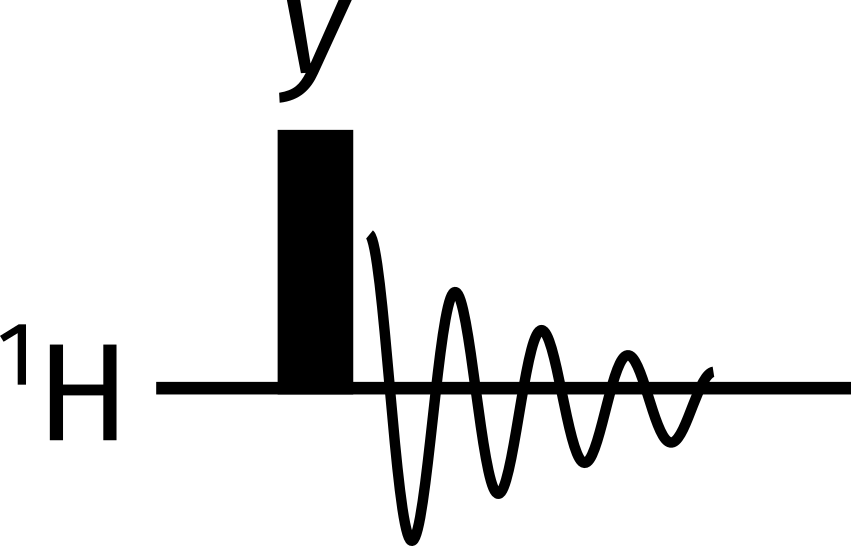
\includegraphics[]{pp/zg_y.png}%
    \caption[Pulse--acquire experiment]{1D \proton{} pulse--acquire experiment.}
\end{figure}

To understand this, we begin with the thermal density operator $\rho_0' = I_z$ (\cref{eq:rho0_simplified}) and assume that there is only one spin in the sample, and that the pulse is applied on-resonance.
The corresponding Hamiltonian during the pulse is simply $\omega_1 I_y$ (\cref{eq:hard_pulse_onresonance}).
If the duration of the pulse is $\taup$, then the density operator immediately following the pulse is given by:
\begin{equation}
    \label{eq:rho_after_pulse}
    \rho = \exp(-\mi\omega_1 I_y\taup) I_z \exp(\mi\omega_1 I_y\taup) = \cos(\omega_1\taup)I_z + \sin(\omega_1\taup)I_x.
\end{equation}
In this case, to obtain a \ang{90} pulse, $\taup$ is specifically calibrated to ensure that $\omega_1\taup = \pi/2$, which yields
\begin{equation}
    \label{eq:rho_after_pulse_simplified}
    \rho = I_x.
\end{equation}
During the detection period, this term evolves under $H_\text{free} = H_\text{cs} = \omega_0 I_z$.
(We use the Schr\"odinger-picture free Hamiltonian here because the measurement of the NMR signal takes place in the laboratory frame.)
At a time $t$ after detection has begun, the density operator is thus:
\begin{equation}
    \label{eq:rho_during_detection}
    \rho(t) = \exp(-\mi \omega_0 I_z t)I_x\exp(\mi\omega_0 I_z t) = \cos(\omega_0 t)I_x + \sin(\omega_0 t)I_y.
\end{equation}
The NMR signal derives from both $x$- and $y$-magnetisation ($M_x$ and $M_y$), which are in turn proportional to $I_x$ and $I_y$ by a factor of $\gamma$.
(If multiple spins are present, then each spin induces its own magnetisation: we would have that $M_x = \sum_i \gamma_i I_{ix}$, and likewise for $M_y$.)
These are then combined to form a complex signal (this process is known as \textit{quadrature detection}):
\begin{align}
    s(t) &= M_x(t) + \mi M_y(t) \label{eq:quadrature} \\
         &\propto \langle I_x(t) \rangle + \mi \langle I_y(t) \rangle \notag \\
         &= \Tr[I_x\rho(t)] + \mi \Tr[I_y\rho(t)] \notag \\
         &\propto \cos(\omega_0 t) + \mi \sin(\omega_0 t) \notag \\
         &= \exp(\mi \omega_0 t). \label{eq:fid}
\end{align}
Before the signal is digitised, the NMR spectrometer mixes this with a \textit{reference} RF field oscillating at the transmitter frequency $\omega_\text{tx}$.
This results in downconversion of the detected frequencies by $\omega_\text{tx}$, such that the actual digitised signal oscillates at the offset frequency $\Omega$ rather than $\omega_0$ (recall we have chosen $\omega_\text{rot} = \omega_\text{tx}$, so $\omega_0 - \omega_\text{tx} = \omega_0 - \omega_\text{rot} = \Omega$).
Therefore, instead of \cref{eq:fid}, the signal we really see is:
\begin{equation}
    \label{eq:fid_reduced}
    s(t) \propto \exp(\mi \Omega t).
\end{equation}
This result is the same as if we had pretended that during the detection period, $\rho$ evolved under the \textit{interaction-picture} free Hamiltonian $H_{\text{free},I} = H_\text{offset}$; we will henceforth adopt this simplification, even though it is not physically accurate.

In practice, relaxation causes this signal to decay with time; this is frequently modelled as an exponential, in accordance with the Bloch equations\autocite{Bloch1946PR}:
\begin{equation}
    \label{eq:fid_with_relaxation}
    s(t) = \exp(\mi\Omega t)\exp(-t/T_2),
\end{equation}
where $T_2$ is the transverse relaxation time.\footnote{Transverse (and longitudinal) relaxation are sometimes called spin--spin (and spin--lattice) relaxation, although the continued usage of these terms has been criticised\autocite{Levitt2008,Keeler2010,Gupta2021JPCL}.}
The NMR signal is thus often called a \textit{free induction decay} (FID).
Fourier transformation of the FID then yields a spectrum with absorption- and dispersion-mode lineshapes in the real and imaginary parts respectively (\cref{fig:lorentzians}):
\begin{equation}
    \label{eq:lorentzian}
    S(\omega) = \mathcal{F}[s(t)] =
    \underbrace{\frac{k}{k^2 + (\omega - \Omega)^2}}_{A(\omega; \Omega)}
    +\, \mathrm{i}\underbrace{\frac{\Omega - \omega}{k^2 + (\omega - \Omega)^2}}_{D(\omega; \Omega)},
\end{equation}
where $k = 1/T_2$.
The notation $A(\omega; \Omega)$ here means that the spectrum is a function of the frequency $\omega$, but is parametrised by the peak offset $\Omega$.
Conventionally, only the real part of the spectrum is displayed, so it is desirable for the real part to contain the absorption-mode lineshape.
This provides better resolution due to the narrower lineshape, and is also less affected by cancellation when multiple peaks overlap.

\begin{figure}[htbp]
    \centering
    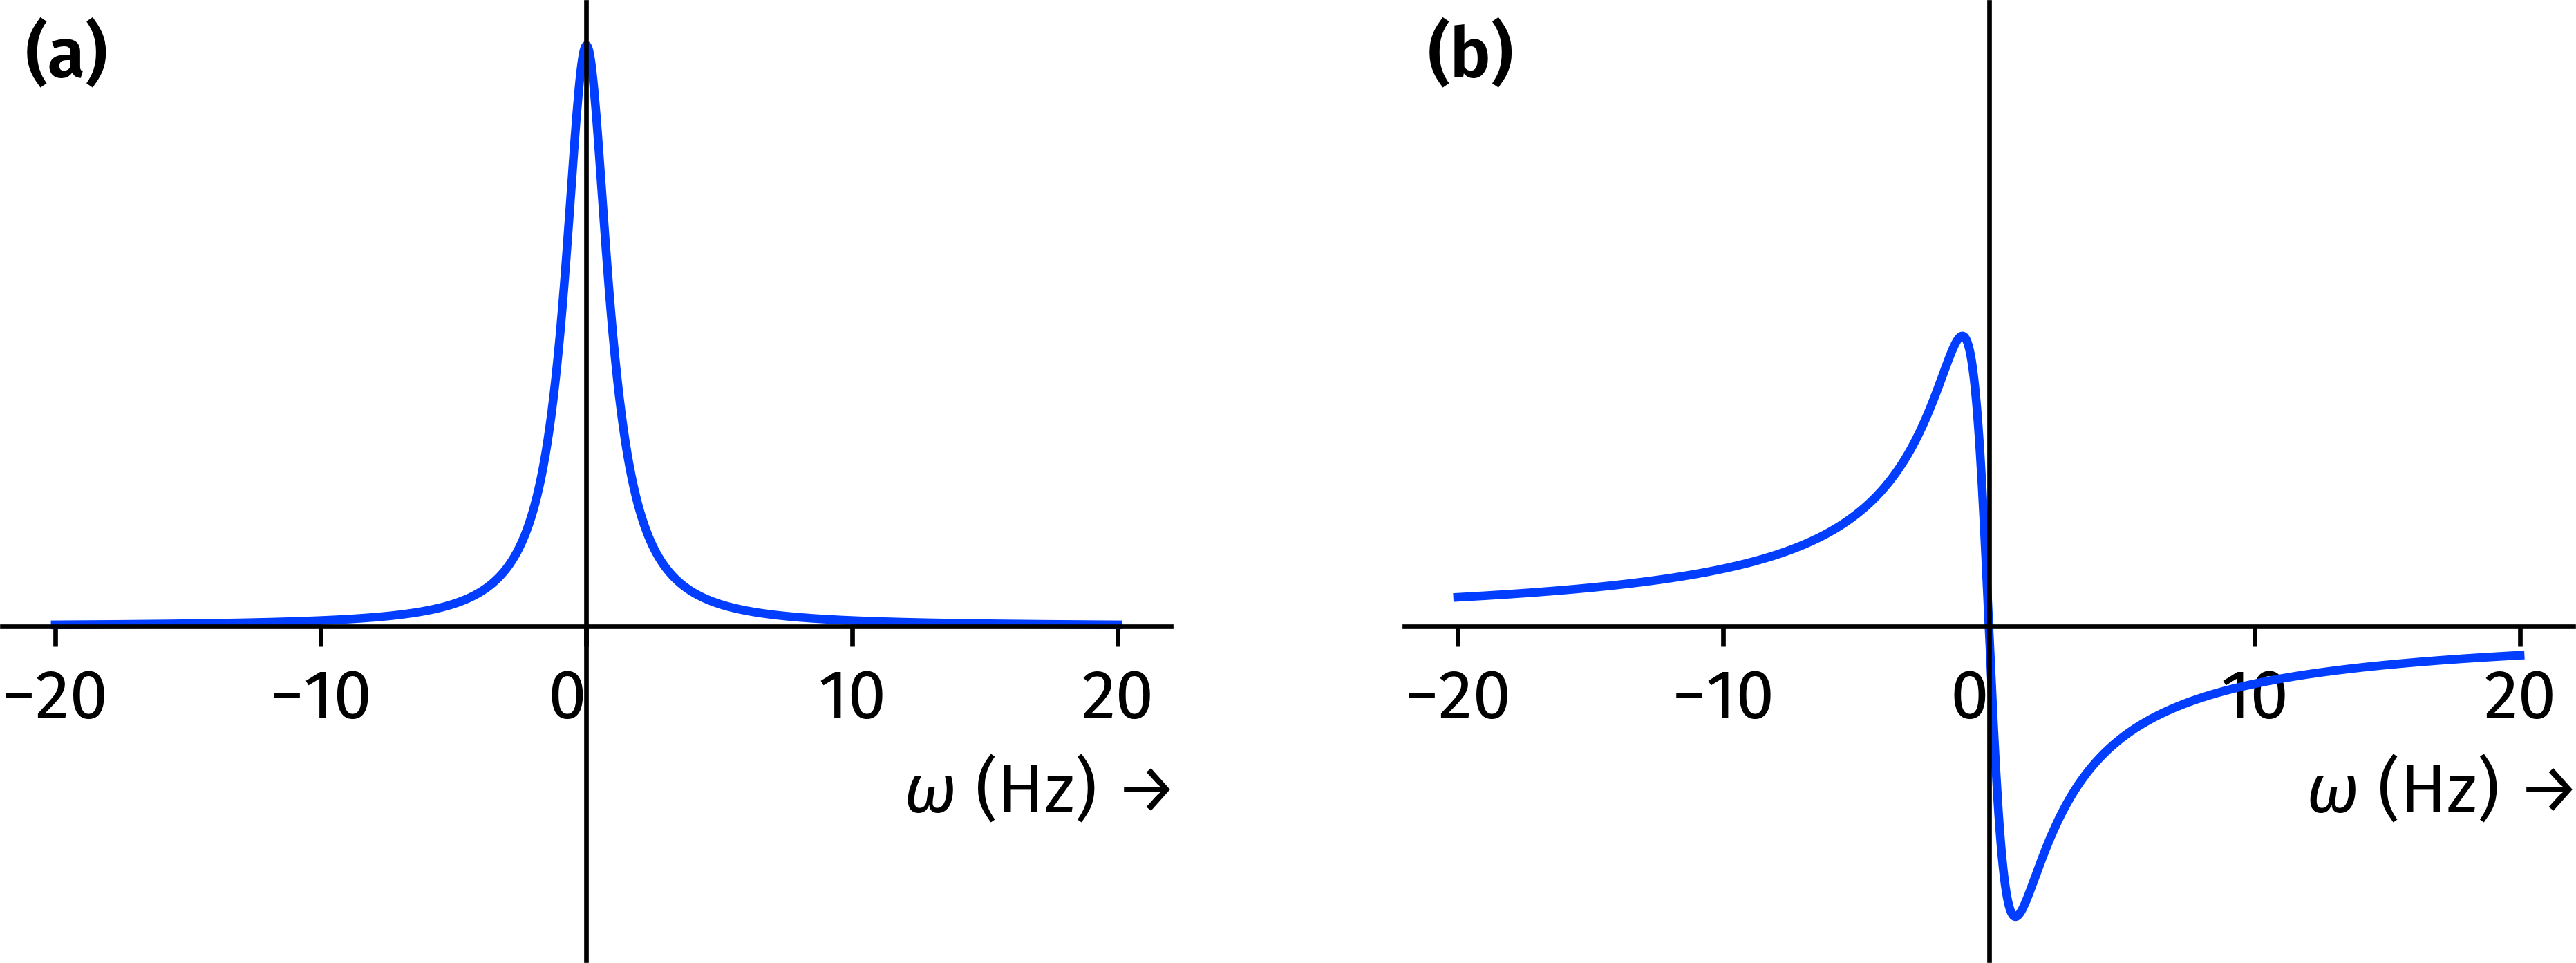
\includegraphics[]{theory/lorentzians.png}%
    {\phantomsubcaption\label{fig:lorentzians_absorption}}%
    {\phantomsubcaption\label{fig:lorentzians_dispersion}}%
    \caption[Absorption- and dispersion-mode Lorentzian lineshapes]{
        \textbf{(\subref{fig:lorentzians_absorption})} Absorption-mode lineshape $A(\omega; \Omega = 0)$.
        \textbf{(\subref{fig:lorentzians_dispersion})} Dispersion-mode lineshape $D(\omega; \Omega = 0)$.
        Both lines have been plotted using $k = \qty{\pi}{\radian\per\second}$.
    }
    \label{fig:lorentzians}
\end{figure}

Strictly speaking, the Lorentzian lineshapes above are only obtained when there is nonzero relaxation during the FID.
For example, in the limit $k \to 0$, $A(\omega; \Omega)$ tends to a delta function $\delta(\omega = \Omega)$.
However, for simplicity, in this thesis I will drop the relaxation term $\exp(-kt)$ unless absolutely necessary; I will simply pretend that a signal of the form $s(t) = \exp(\mi \Omega t)$ is directly Fourier transformed to give $A(\omega; \Omega) + \mi D(\omega; \Omega)$.

Consider now changing the initial pulse such that it is applied along the $+x$-axis instead ($\phi = 0$).
Repeating the above analysis, we find that the resulting signal will have a phase shift:
\begin{align}
    \label{eq:fid_phase_shifted}
    s'(t) &= -\mi\exp(\mi\Omega t) \\
    \Rightarrow \quad S'(\omega) &= \mathcal{F}[s'(t)] = D(\omega;\Omega) - \mi A(\omega;\Omega).
\end{align}
If we were to take the real part of the spectrum here, then we would obtain the undesired dispersion-mode lineshape $D(\omega;\Omega)$.
There are two ways of removing this phase shift.
The first is to shift the \textit{receiver phase} by $\phi_\text{rec}$, which introduces an extra factor of $\exp(-\mi\phi_\text{rec})$ to the detected signal: we can thus choose $\phi_\text{rec} = 3\pi/2$ in order to cancel out the $-\mi$ term in $s'(t)$.
Alternatively, the spectrum can be processed through \textit{phase correction}, in which $S(\omega)$ is directly multiplied by a term $\exp(\mi\phi_\text{corr})$, where $\phi_\text{corr}$ is a linear function of the frequency $\omega$:
\begin{equation}
    \label{eq:phase_correction}
    \phi_\text{corr} = \phi_{\text{corr}}^{(0)} + \omega\phi_{\text{corr}}^{(1)}.
\end{equation}
$\phi_\text{corr}^{(0)}$ and $\phi_\text{corr}^{(1)}$ are respectively termed the \textit{zeroth-} and \textit{first-order phase corrections}: in this idealised case, we can simply choose $(\phi_\text{corr}^{(0)}, \phi_\text{corr}^{(1)}) = (\pi/2, 0)$ to again remove the unwanted phase shift.
More realistically, due to instrumental imperfections, both of these values will have to be nonzero in order to ensure that every peak in the spectrum has the correct phase, i.e.\ is displayed in absorption-mode.

An alternative framework for analysing pulse sequences is to use the ladder operators $I_+$ and $I_-$ (\cref{eq:other_single_spin_ops}).
Using the original example with our initial pulse on $+y$, the density operator immediately after the pulse is:
\begin{equation}
    \label{eq:rho_coherences}
    \rho = I_x = \frac{1}{2}(I_+ + I_-),
\end{equation}
and during detection this evolves as:
\begin{equation}
    \label{eq:fid_coherences}
    \rho(t) = \cos(\Omega t)I_x + \sin(\Omega t)I_y = \frac{1}{2}\left[\exp(-\mi \Omega t)I_+ + \exp(\mi \Omega t)I_- \right].
\end{equation}
(Notice that the $+1$-coherence $I_+$ actually evolves at the negative frequency $-\Omega$.)
To obtain the same signal as previously done in \cref{eq:fid}, we `detect' the $I_-$ term:
\begin{equation}
    \label{eq:detection_coherences}
    s(t) \propto \Tr[I_- \rho(t)] \propto \exp(\mi\Omega t),
\end{equation}
which leads to the common assertion that \textit{only quantum coherences of order $-1$ are detectable}.
It is true that coherences with orders $p = 0, \pm 2, \pm 3, \ldots$ can never be detected in an FID.
However, it is worth pointing out that the `uniqueness' of $-1$-coherence is merely a result of how the $x$- and $y$-magnetisation are combined to form the complex signal (\cref{eq:quadrature}).
We do not \textit{physically} detect $I_-$: we detect $I_x$ and $I_y$, and combine them to form a complex signal which is mathematically equal to detecting $I_-$.
If we had instead chosen to combine them in a different way, such as $s(t) = M_x(t) - \mi M_y(t)$, this would give us $s(t) \propto \exp(-\mi\Omega t)$---corresponding to `detection' of $+1$-coherence---although this alternative does come with the drawback that frequencies must be reversed after Fourier transformation.
In any case, we will stick to the established convention of detecting $-1$-coherence here.

To end this section, it should be pointed out that the complex signal is not obtained as an infinitely-long, continuous function of time, as the treatment above implies.
The complex-valued signal is digitised at an interval called the \textit{dwell time}, $\tau_\text{dw}$, and detection must be stopped after a finite period called the \textit{acquisition time}, $\tau_\text{aq}$.
The FT being performed is actually a discrete Fourier transform (DFT), which yields a periodic function $S(\omega)$; its period (in Hz) is given by $1/\tau_\text{dw}$.%
\footnote{The periodicity property of the DFT is equivalent to the Nyquist theorem, which is usually formulated as follows: the sampling rate required to correctly digitise a signal containing frequencies in the range $[0, f_\text{max}]$ is $1/(2f_\text{max})$. In the main text, it appears as if we have dropped the factor of $2$ in the denominator; but in truth this statement of the Nyquist theorem is applicable to \textit{real-valued} signals, and here we have a \textit{complex-valued} signal $s(t)$, which effectively doubles the range of correctly sampled frequencies.}
The NMR spectrum displayed to the user corresponds to one single period of $S(\omega)$, and thus the \textit{spectral width} is also equal to $1/\tau_\text{dw}$.%
\footnote{Frustratingly, the \texttt{DW} parameter in Bruker's TopSpin software is actually equal to $\tau_\text{dw}/2$. The reason is because this parameter corresponds to the interval between which \textit{real} data is sampled, which is effectively twice as fast as complex-valued sampling.}
In principle, the periodicity of the DFT means that signals which would ordinarily fall outside of the spectral width would appear at incorrect frequencies in the spectrum.\autocite{Turner1986JMR}
On modern instrumentation, this is no longer the case for direct detection; peaks outside of the spectral width are removed using digital filters.
However, \textit{folding} or \textit{aliasing} of peaks in the indirect dimension(s) of multidimensional NMR spectra still occurs.

The DFT $S(\omega)$ is also a discrete function itself, and its resolution is given by $1/\tau_\text{aq}$.
It is possible to extend the effective acquisition time (and thus improve spectral resolution) without actually acquiring more data: this can be done either by \textit{forward linear prediction} of the signal, or by simply adding zeros onto the end of the signal (\textit{zero-filling}).


\subsection{INEPT and product operators}
\label{subsec:theory__inept}

\begin{figure}[htbp]
    \centering
    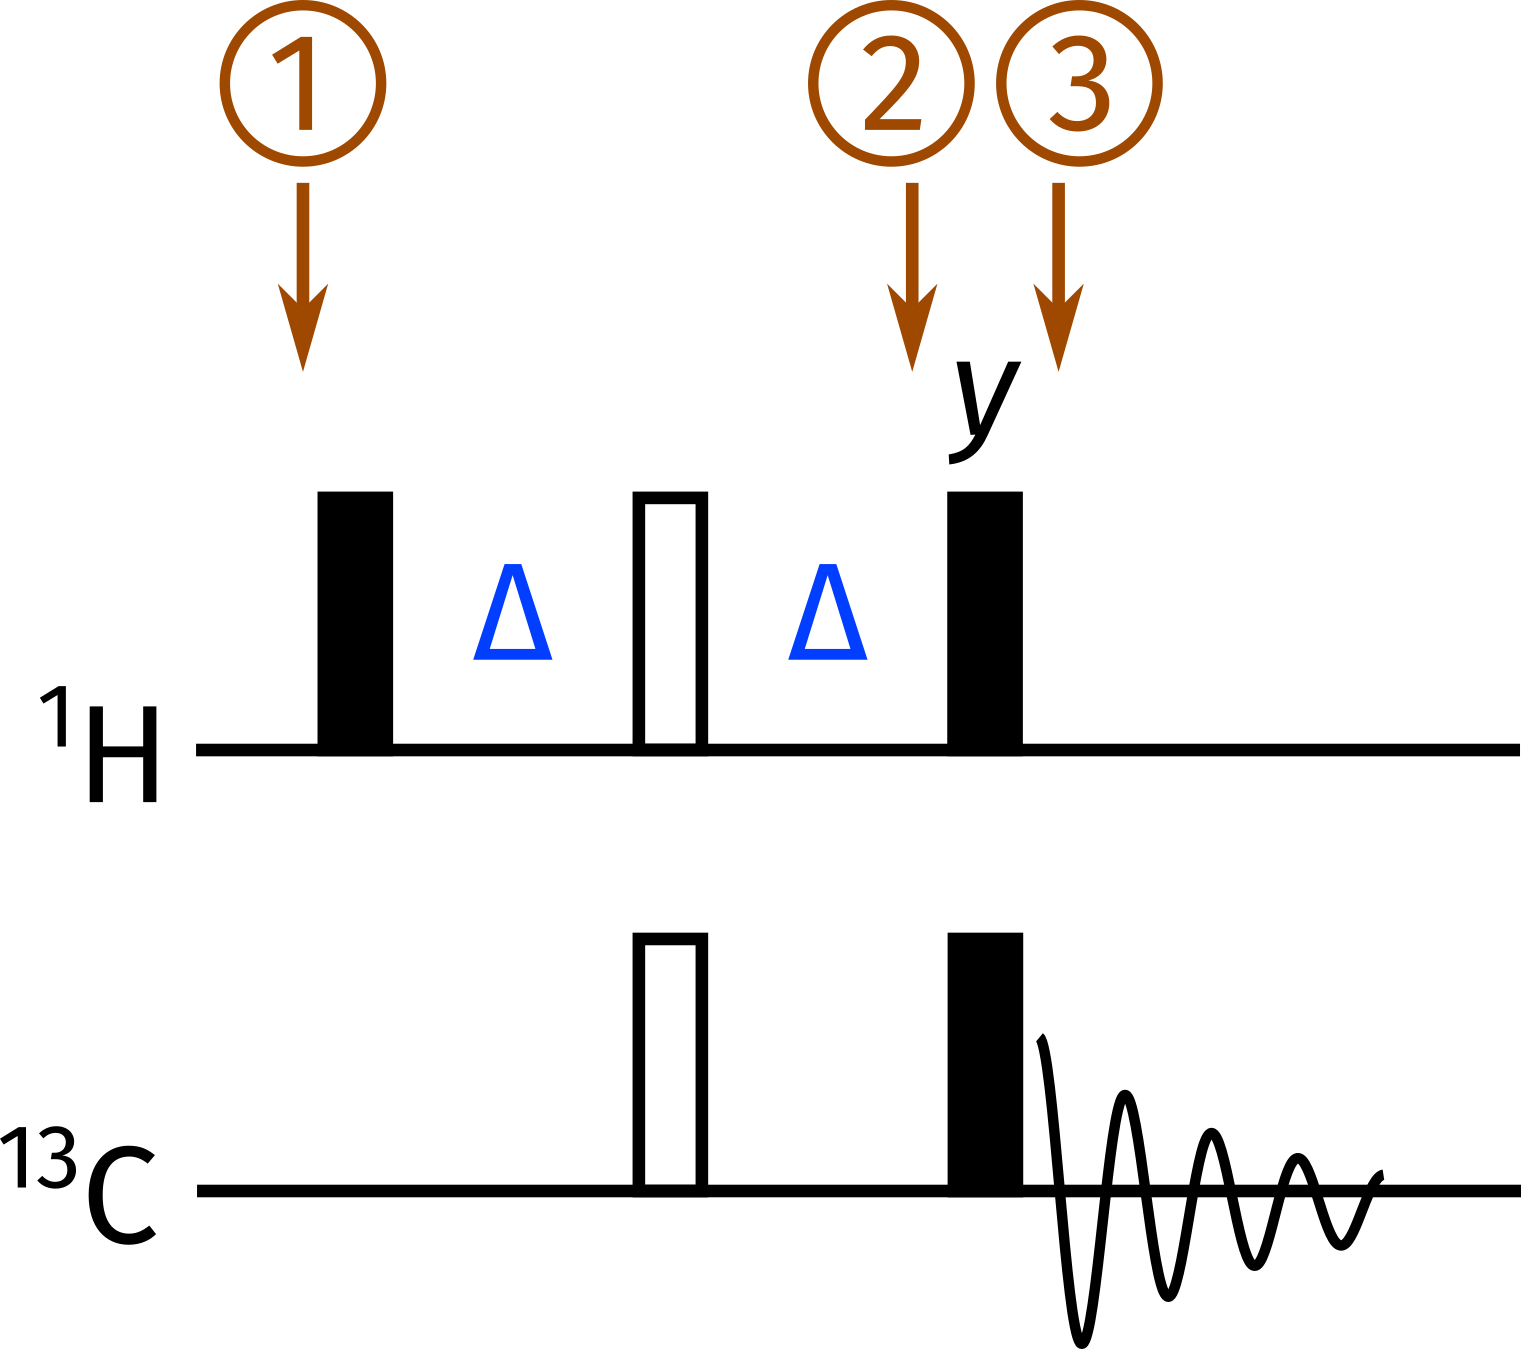
\includegraphics[]{pp/inept.png}%
    \caption[INEPT pulse sequence]{
        INEPT pulse sequence.
        The delay $\Delta$ is set to $1/(4 \cdot \oneJ{CH})$.
    }
    \label{fig:inept}
\end{figure}

Having tackled a simple single-spin case, we now move to the analysis of coupled spin systems and the development of the so-called `product operator formalism'.\autocite{Sorensen1984PNMRS}
In particular, we look at the INEPT experiment\autocite{Morris1979JACS,Morris1980JACS}, in which magnetisation is transferred from a a nuclide with a high magnetogyric ratio to one with a low magnetogyric ratio through a scalar coupling: for example, from \proton{} to \carbon{} using the one-bond coupling constant, $\oneJ{CH}$ (\cref{fig:inept}).
Following tradition, the two nuclei are respectively labelled $I\/$ and $S$.%
\footnote{This may seem insensible since $I\/$ is the \textit{sensitive} and $S$ the \textit{insensitive} nucleus, and indeed, in the original literature\autocite{Morris1979JACS} the meanings of $I\/$ and $S$ were swapped. However, this usage has not been consistent\autocite{Pines1972JCP}, and in modern usage the identification of $I\/$ as the sensitive nucleus seems to have prevailed.}
The Schr\"odinger-picture free Hamiltonian for a weakly coupled system (cf.\ \cref{eq:weak_coupling,eq:h_j_secular}) is $H_\text{free} = \omega_{0,I} I_z + \omega_{0,S} S_z + 2\pi J_{IS} I_z S_z$.
At the very beginning of the sequence (point \circled{1}), we formally have the equilibrium density operator
\begin{equation}
    \label{eq:density_eqm_heteronuclear_full}
    \rho_0 = \frac{\exp(-\beta\hbar H_\text{free})}{\Tr[\exp(-\beta\hbar H_\text{free})]}
    \approx E - \beta\hbar (\omega_{0,I} I_z + \omega_{0,S} S_z + 2\pi J_{IS} I_z S_z),
\end{equation}
using the same approximations as in \cref{eq:nmr_equilibrium_rho}.
The scalar coupling term can be safely neglected as $2\pi J_{IS}$ is several orders of magnitude smaller than the Larmor frequencies $\omega_0$.
After removing the physically irrelevant $E\/$ term and factoring out a constant of $\beta\hbar B_0$, we end up with:
\begin{equation}
    \label{eq:density_eqm_heteronuclear_simplified}
    \rho'_0 = \gamma_I I_z + \gamma_S S_z.
\end{equation}
This represents equilibrium magnetisation (or \textit{polarisation}) on both spins $I\/$ and $S$, in proportion to their magnetogyric ratios.
In general, an NMR experiment may manipulate---and ultimately detect---both of these terms.
Since unitary evolution according to the Liouville--von Neumann equation is \textit{linear}, in that $U(\rho_1 + \rho_2)\adj{U} = U\rho_1\adj{U} + U\rho_2\adj{U}$, we can treat these two terms separately: we focus first on the spin-$I\/$ polarisation, $\rho_I = \gamma_I I_z$.
The first $90^\circ_x$ \proton{} pulse tips this magnetisation into the transverse plane (ignoring off-resonance effects):
\begin{equation}
    \label{eq:rho_after_pulse_x}
    \rho_I \to \exp[-\mi(\pi/2) I_x] \gamma_I I_z \exp[\mi(\pi/2) I_x] = -\gamma_I I_y.
\end{equation}
In principle, we could continue in this manner through repeated application of the `sandwich' formulae (\cref{eq:sandwich_formula_1,eq:sandwich_formula_2}, as well as an analogous version for the $I_zS_z$ term). 
For example, in the $\Delta$ delay which follows, we have that
\begin{equation}
    \label{eq:rho_after_delay_x}
    \begin{aligned}
        \rho_I &\to -\gamma_I\exp(-\mi H_{\text{free},I} \Delta) I_y \exp(\mi H_{\text{free},I} \Delta) \\
               &= -\gamma_I\exp(-\mi H_\text{J} \Delta)\exp(-\mi H_\text{offset}\Delta) I_y \exp(\mi H_\text{offset} \Delta)\exp(\mi H_\text{J}\Delta) \\
               &= \ldots
    \end{aligned}
\end{equation}
When performing simulations of NMR experiments, such as those in later chapters, this is precisely what happens, with the slight difference that the Liouville--von Neumann equation (\cref{eq:lvn_interaction_integrated}) is evaluated numerically rather than symbolically.
Note that in going from the first to the second line, we can only `split up' $H_{\text{free},I}$ into its constituent components $H_\text{offset}$ and $H_\text{J}$ because they commute.

\begin{figure}[htbp]
    \centering
    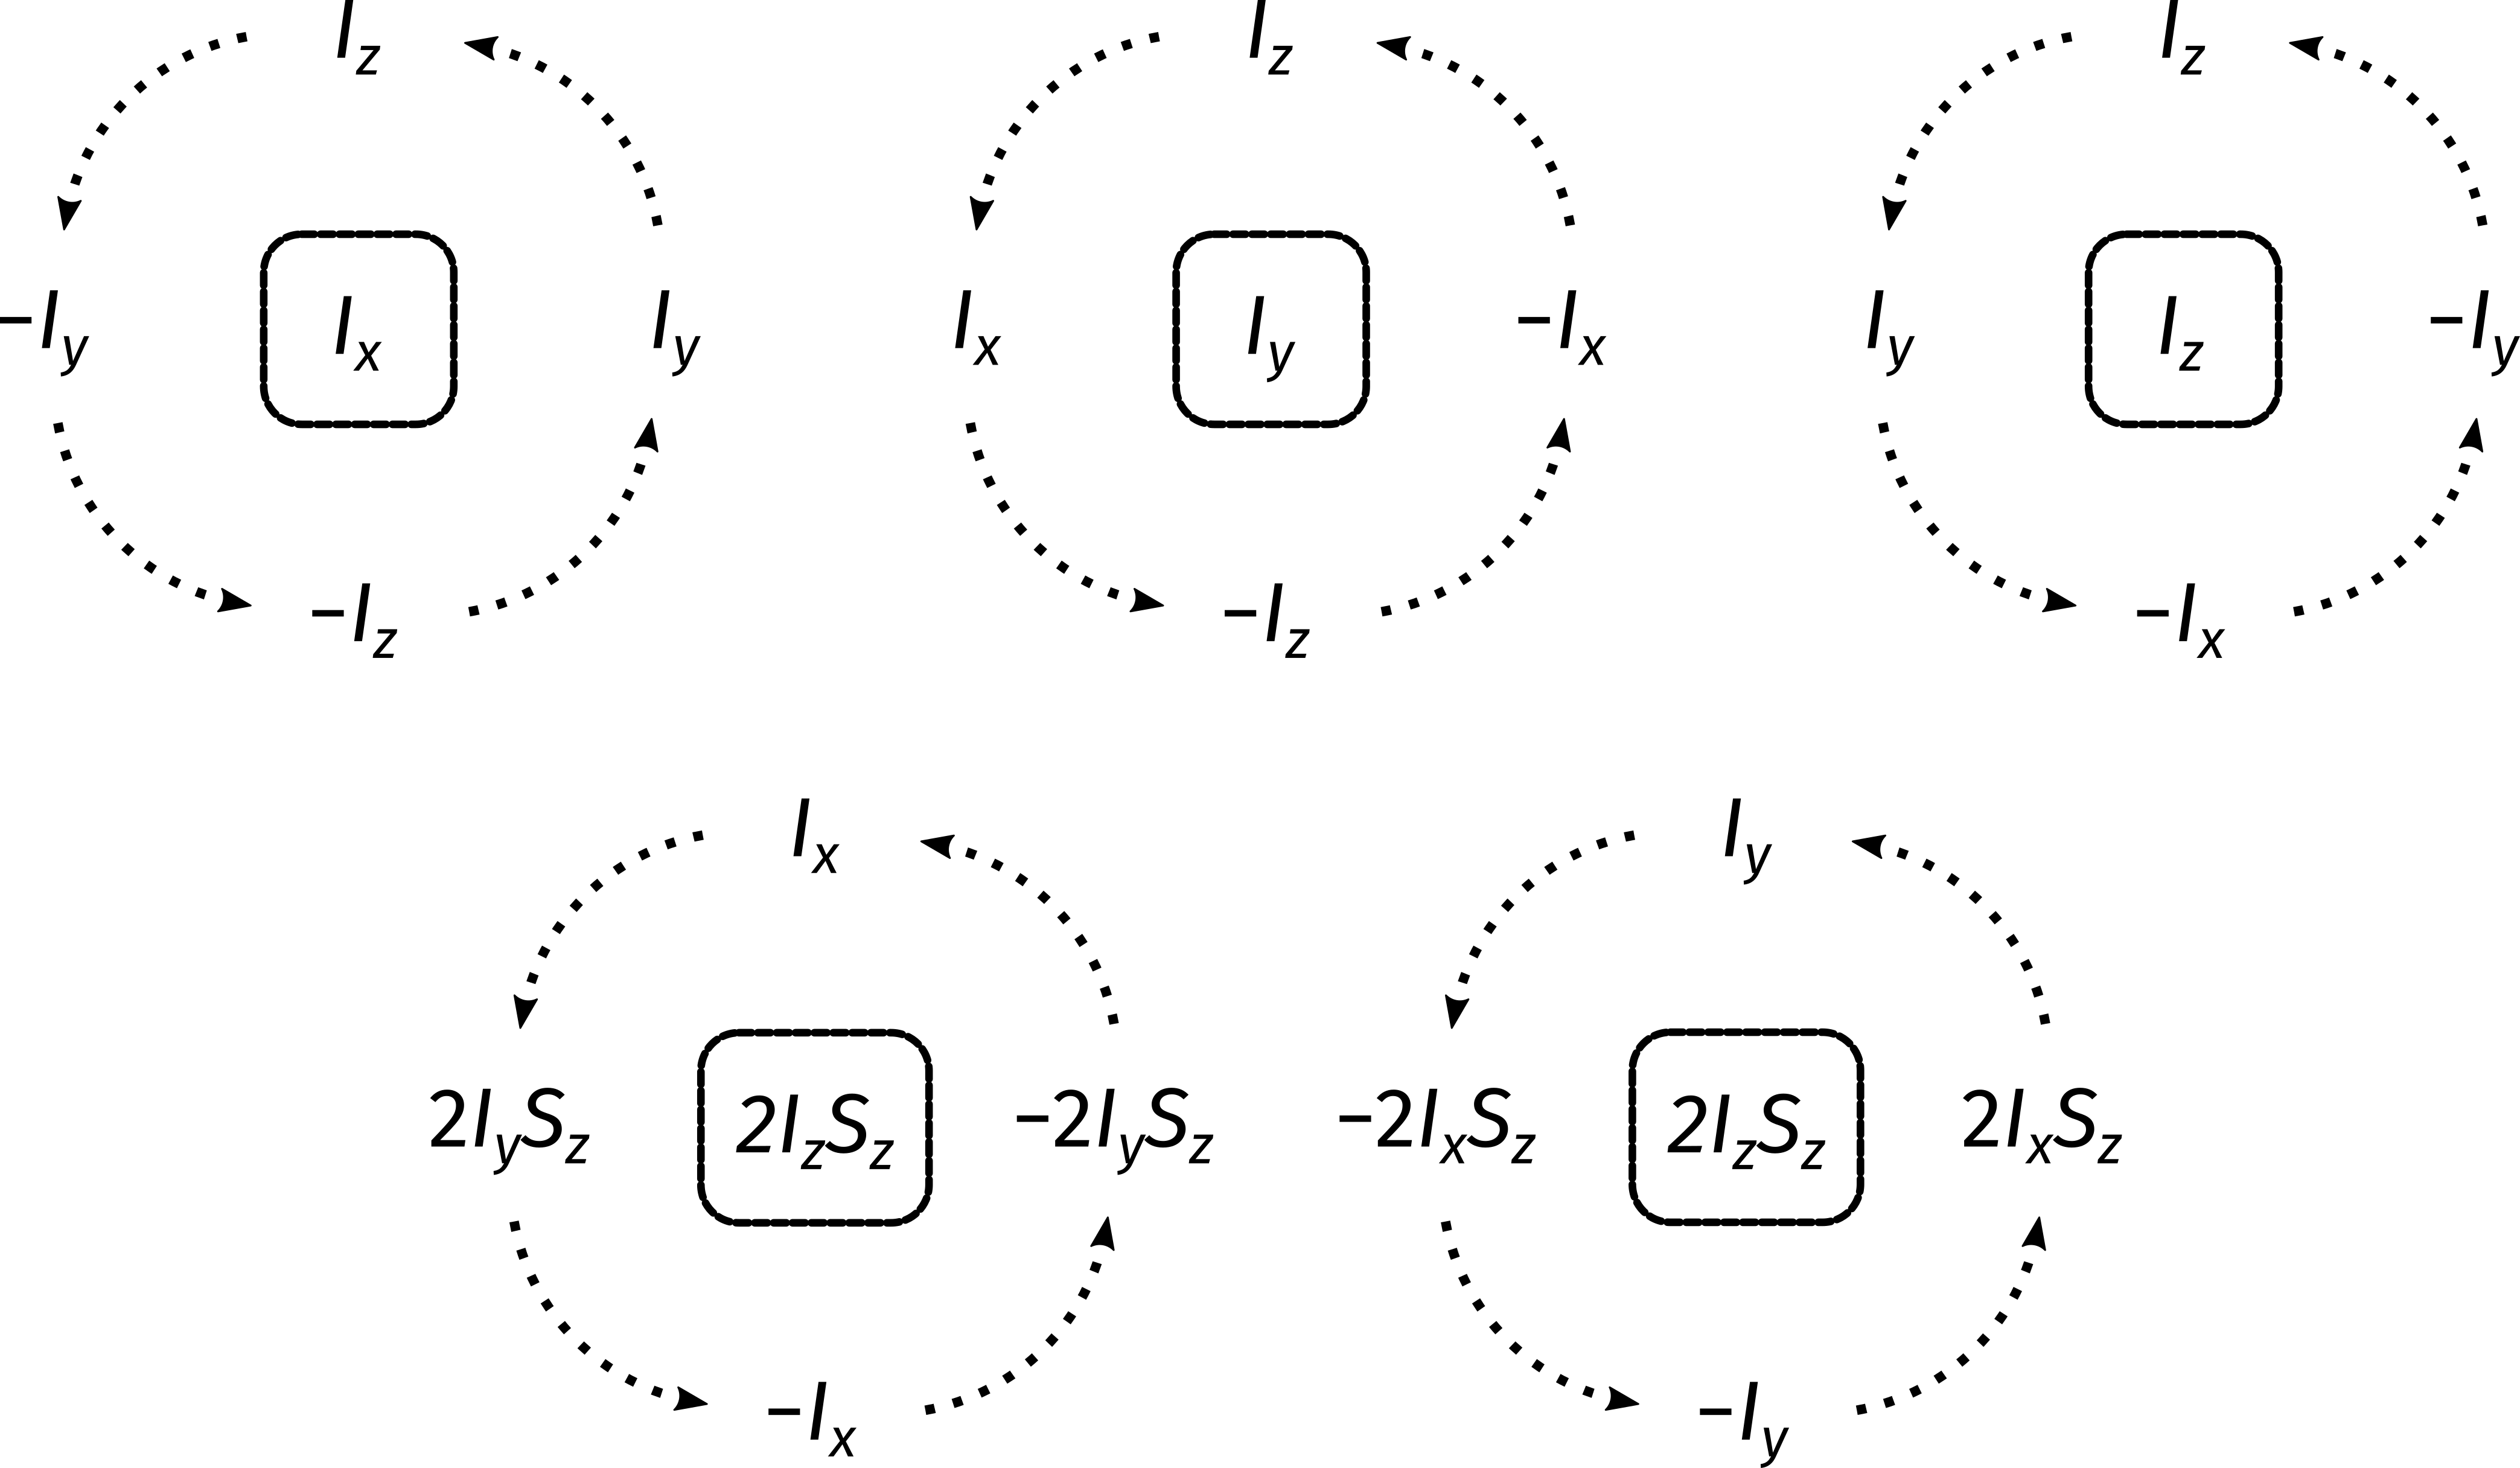
\includegraphics[]{theory/prodop_rules.png}%
    \caption[Simplified rules for product operator evolutions]{
        Simplified rules for the evolution of product operators under different common Hamiltonians (offset, weak/secular J-coupling, and pulses).
        These Hamiltonians often have the form $\omega M$ where $M$ is some `base operator', and are applied for a time $\tau$.
        The boxed operators in the centre of each group refer to $M$; the initial state is then `rotated' about this by an angle of $\omega\tau$ to obtain the final state, or more formally, it is transformed into itself times $\cos(\omega\tau)$, plus the next term in the cycle times $\sin(\omega\tau)$.
        For example, an $90^\circ_x$ pulse has the `base' operator $I_x$ and the angle $\omega\tau = \pi/2$; thus, the initial state $I_z$ would be rotated to $I_z\cos(\pi/2) - I_y\sin(\pi/2) = -I_y$.
    }
    \label{fig:prodop_rules}
\end{figure}

When analysing pulse sequences by hand, however, it is far more convenient to use a set of heuristics which summarise the effects of various pulse sequence elements.
For example, \cref{fig:prodop_rules} summarises the evolution of a density operator under a single term of the Hamiltonian: as above, since $[H_\text{offset}, H_\text{J}] = 0$, we only need to consider one term at a time.
More high-level rules may be devised as well: for example, during the $\Delta\text{--}180^\circ_{x}(I),180^\circ_{x}(S)\text{--}\Delta$ spin echo which comes next, the $J_{IS}$ interaction in $H_{\text{free},I}$ is allowed to evolve for a period of $2\Delta$, but the offset term is \textit{refocused} and can be ignored.
(The sign inversion caused by the \ang{180} pulses must also be included.)
As per \cref{fig:prodop_rules}, this transforms the $-I_y$ term to $-2I_xS_z$ at point \circled{2}: the Hamiltonian is $\pi J_{IS} 2I_zS_z$ for a total time of $2\Delta = 1/(2J_{IS})$, so the `angle' rotated through is $\pi J_{IS}/(2J_{IS}) = \pi/2$.
Immediately after this, the $90^\circ_y(I),90^\circ_x(S)$ pair of pulses rotates this magnetisation to $-2I_zS_y$ (point \circled{3}).
These transformations are often denoted with simpler notation:
\begin{equation}
    \label{eq:inept_prodop}
    \gamma_I I_z
    \xrightarrow{90^\circ_x(I)} -\gamma_I I_y
    \xrightarrow{\Delta\text{--}180^\circ_{x}(I),180^\circ_{x}(S)\text{--}\Delta} -2\gamma_I I_xS_z
    \xrightarrow{90^\circ_y(I),90^\circ_x(S)} -2\gamma_I I_zS_y
\end{equation}
During the detection period, the term $-2\gamma_II_zS_y$ evolves as
\begin{align}
    \label{eq:inept_fid_prodop}
    -2\gamma_I I_zS_y \xrightarrow{H_{\text{free},I}} -2\gamma_I I_zS_y\cos(\Omega_St)\cos(\pi Jt) + \gamma_I S_x\cos(\Omega_St)\sin(\pi Jt) \notag{} \\
    \qquad {} - 2\gamma_I I_zS_x\sin(\Omega_St)\cos(\pi Jt) + \gamma_I S_y\sin(\Omega_S t)\sin(\pi Jt),
\end{align}
from which we extract the complex signal
\begin{equation}
    \label{eq:inept_fid}
    s_I(t) = \langle S_x(t) \rangle + \mi \langle S_y(t) \rangle = \frac{\gamma_I}{2\mi}\bigl\{\exp[\mi(\Omega_S + \pi J_{IS})t] - \exp[\mi(\Omega_S - \pi J_{IS})t]\bigr\}.
\end{equation}
After Fourier transformation, the resulting spectrum has two peaks with opposite phase and have the frequencies $\Omega_S \pm \pi J_{IS}$; because of the factor of $1/(2\mi)$, the real part of the spectrum will contain dispersion-mode signals (\cref{fig:doublet_lorentzians_dis_anti}).
If desired, zeroth-order phase correction can be performed here, yielding instead a pair of absorption-mode signals still with opposite phases (\cref{fig:doublet_lorentzians_abs_anti}).
In either case, this is termed an \textit{antiphase} doublet; the product operators which give rise to it ($2I_zS_x$ and $2I_zS_y$) are said to be antiphase with respect to spin $I\/$.
Importantly, the amplitude of the signal scales as $\gamma_I$ rather than $\gamma_S$; since $\gamma_I > \gamma_S$, this represents a sensitivity enhancement compared to the direct excitation of $S$-magnetisation.

\begin{figure}[htbp]
    \centering
    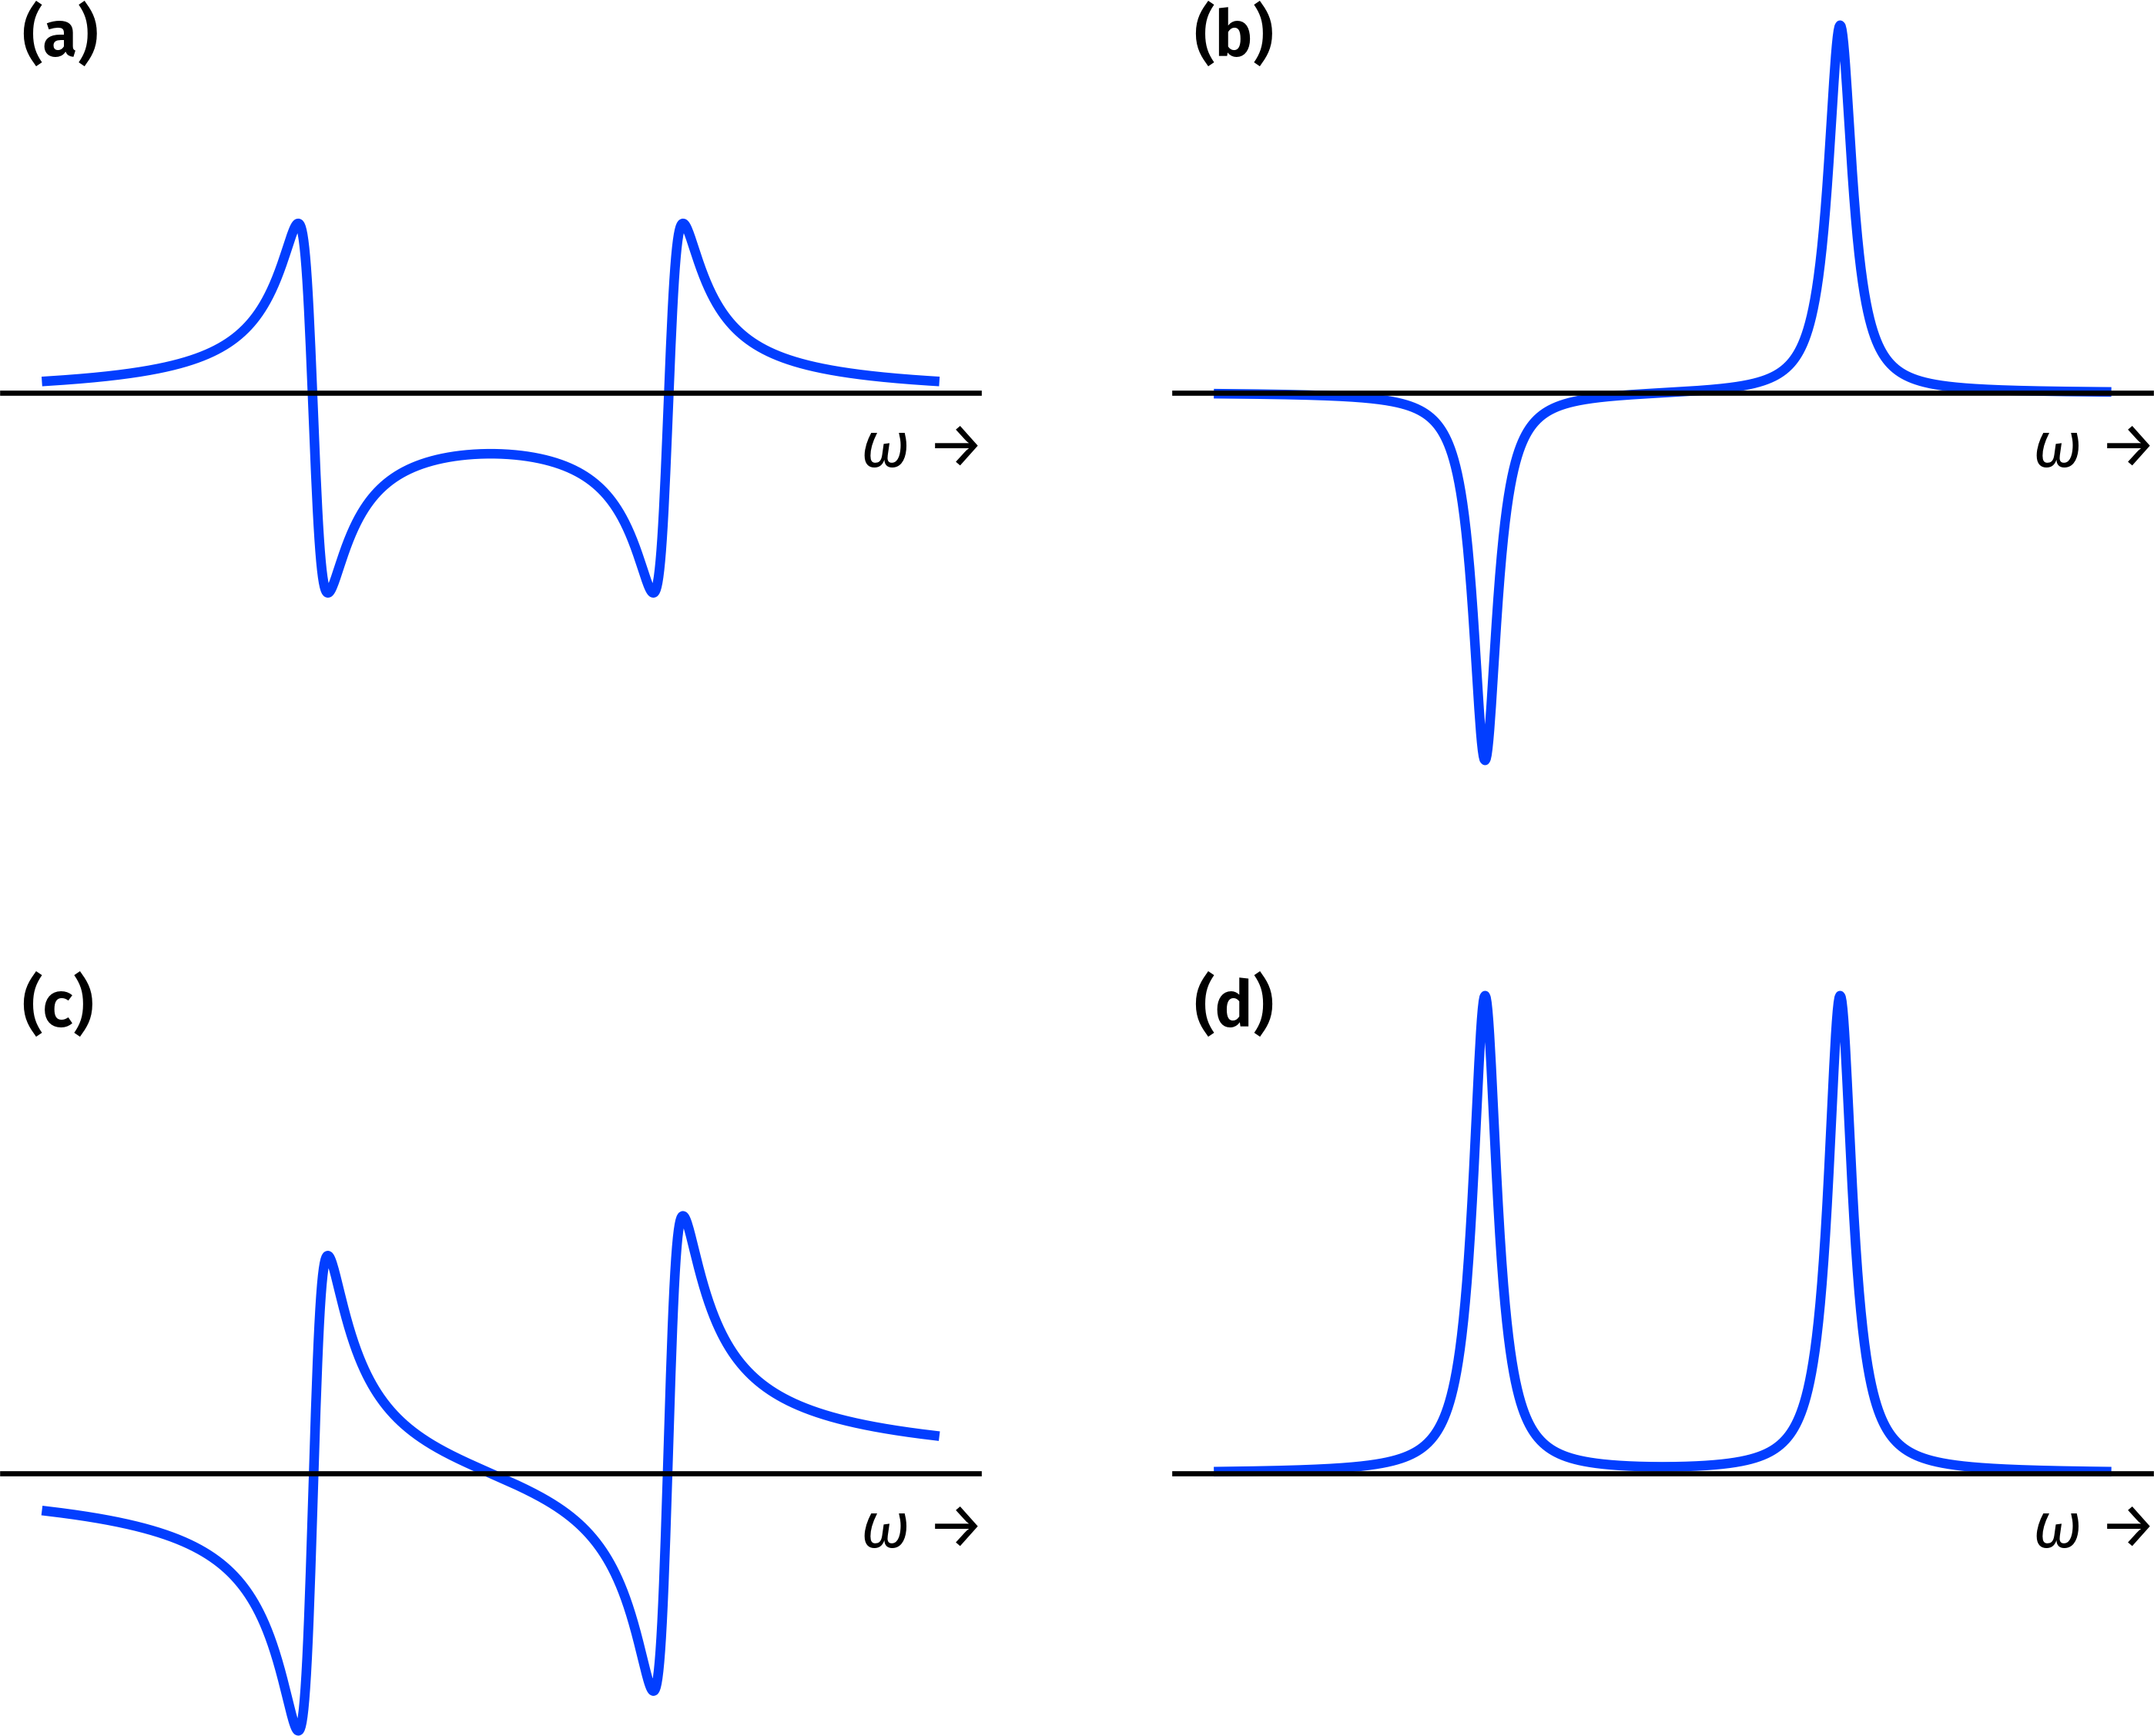
\includegraphics[]{theory/doublet_lorentzians.png}%
    {\phantomsubcaption\label{fig:doublet_lorentzians_dis_anti}}%
    {\phantomsubcaption\label{fig:doublet_lorentzians_abs_anti}}%
    {\phantomsubcaption\label{fig:doublet_lorentzians_dis_in}}%
    {\phantomsubcaption\label{fig:doublet_lorentzians_abs_in}}%
    \caption[Absorption- and dispersion-mode in-phase and antiphase doublets]{
        Peak shapes of a doublet.
        In all cases, the separation between the two peaks is $2\pi J_{IS}$.
        \textbf{(\subref*{fig:doublet_lorentzians_dis_anti})} Antiphase, dispersion-mode.
        \textbf{(\subref*{fig:doublet_lorentzians_abs_anti})} Antiphase, absorption-mode.
        \textbf{(\subref*{fig:doublet_lorentzians_dis_in})} In-phase, dispersion-mode.
        \textbf{(\subref*{fig:doublet_lorentzians_abs_in})} In-phase, absorption-mode.
    }
    \label{fig:doublet_lorentzians}
\end{figure}

Of course, this is only half of the picture; we have not considered what happens to the other part of the magnetisation, namely $\rho_S = \gamma_S S_z$.
Clearly, this is unaffected by the initial $90^\circ_x(I)$ pulse and the first $\Delta$ delay.
The $180^\circ_x(S)$ pulse inverts it, and the final $90^\circ_x(S)$ pulse in fact transforms it into observable $S$-magnetisation:
\begin{equation}
    \label{eq:inept_prodop_s}
    \gamma_S S_z \xrightarrow{90^\circ_x(I)\text{--}\Delta} \gamma_S S_z
    \xrightarrow{180^\circ_x(I),180^\circ_x(S)\text{--}\Delta} -\gamma_S S_z
    \xrightarrow{90^\circ_y(I),90^\circ_x(S)} \gamma_S S_y
\end{equation}
This term produces \textit{in-phase} spin-$S$ magnetisation during the detection period (where the two components of the doublet have the same phase):
\begin{equation}
    \label{eq:inept_fid_S}
    s_S(t) = \frac{\mi\gamma_S}{2}\bigl\{\exp[\mi(\Omega_S + \pi J_{IS})t] + \exp[\mi(\Omega_S - \pi J_{IS})t]\bigr\},
\end{equation}
Because of the factor of $\mi$, the real part of the spectrum will contain a dispersion-mode doublet (\cref{fig:doublet_lorentzians_dis_in}).
The signal actually measured by the spectrometer is $s(t) = s_I(t) + s_S(t)$; and the spectrum is a weighted sum of in-phase and antiphase magnetisation.
This leads to potentially unwanted phase distortions in the spectrum, which one would prefer to suppress.

This can be accomplished through the technique of \textit{phase cycling}, where pulse and receiver phases are changed in concert and the resulting FIDs summed in order to select for a particular signal.
In this case, the INEPT experiment is performed twice, once with the phases as given in \cref{fig:inept}, and once where the initial $90^\circ_x(I)$ pulse is replaced with a $90^\circ_{-x}(I)$ pulse.
The first of these gives us the same signals as above.
However, inverting the initial $I\/$ pulse leads to $s_I$ acquiring a minus sign, because the initial $I_z$ term is rotated to $I_y$ instead of $-I_y$.
On the other hand, the signal component $s_S$ is unaffected by this pulse and thus does not experience a change of sign.
The two FIDs we record are thus as follows:
\begin{align}
    \label{eq:inept_phase_cycling}
    s_1(t) &= s_I(t) + s_S(t) \\
    s_2(t) &= -s_I(t) + s_S(t)
\end{align}
Simply taking the difference of these two FIDs yields a signal where the desired $s_I$ has been accumulated and $s_S$ has been cancelled out.
In practice, instead of subtracting the two signals, it is typical to shift the receiver phase $\phi_\text{rec}$ by \ang{180} in the second experiment: this introduces a phase shift of $\exp(-\mi\pi) = -1$ to the signal, and the two signals can now be \textit{added} together instead of subtracted to cancel out $s_S$.
Since both $\phi_1$ and $\phi_\text{rec}$ are $0$ on the first experiment and $\pi$ on the second experiment, we can express this as $\phi_x = \phi_\text{rec} = (0, \pi)$.
This is more commonly denoted as $\phi_1 = \phi_\text{rec} = (x, -x)$, because the phases $(0, \pi)$ correspond to the $+x$- and $-x$-axes respectively.

The `simplified' analysis of pulse sequences shown in \cref{eq:inept_prodop,eq:inept_prodop_s} is often called \textit{`product operator'} analysis\autocite{Sorensen1984PNMRS}, because the underlying two-spin operators are products of single-spin Cartesian operators.
Although this is often touted as being `simpler' than full density operator calculations, it is really just a shorthand which masks the quantum mechanical theory developed in this chapter:
\begin{equation}
    \label{eq:product_operator_shorthand}
    \underbrace{I_z \xrightarrow{90^\circ_x(I)} -I_y}_{\textit{product operator}}
    \quad\Longleftrightarrow\quad
    \underbrace{\exp(-\mi I_x\pi/2)I_z\exp(\mi I_x\pi/2) = -I_y}_{\textit{density operator}}
\end{equation}
Since the operators $\{E, I_x, I_y, I_z\}$ form a complete basis for a single-spin system, their products (i.e.\ product operators) likewise form a complete basis for multiple-spin systems, and so \textit{any} density matrix for a multiple-spin system may be expressed as a linear combination of product operators.
Strictly speaking, the use of product operators therefore does not actually sacrifice any power in and of itself.
However, the heuristics such as those in \cref{fig:prodop_rules} \textit{are} limiting, in that the evolution under some Hamiltonians---for example, strong coupling $\symbf{I}\cdot\symbf{S}$, or pulses for off-resonance spins where $H\/$ is a sum of $I_x$ and $I_z$---cannot be neatly captured in such a pictorial form.


\subsection{2D NMR: HSQC}
\label{subsec:theory__hsqc}

The use of coherence orders is particularly effective in the analysis of modern 2D NMR experiments, which make use of multiple different techniques to select for particular \textit{coherence transfer pathways} (CTPs).
A full discussion of this is beyond the scope of this thesis.
Nevertheless, the analysis of a 2D \proton{}--\carbon{} HSQC experiment (\cref{fig:hsqc_1grad}) is given here as an example to illustrate the concepts of CTP selection through \textit{phase cycling} and gradients, as well as the related issue of quadrature detection in indirect dimensions.

\begin{figure}[ht]
    \centering
    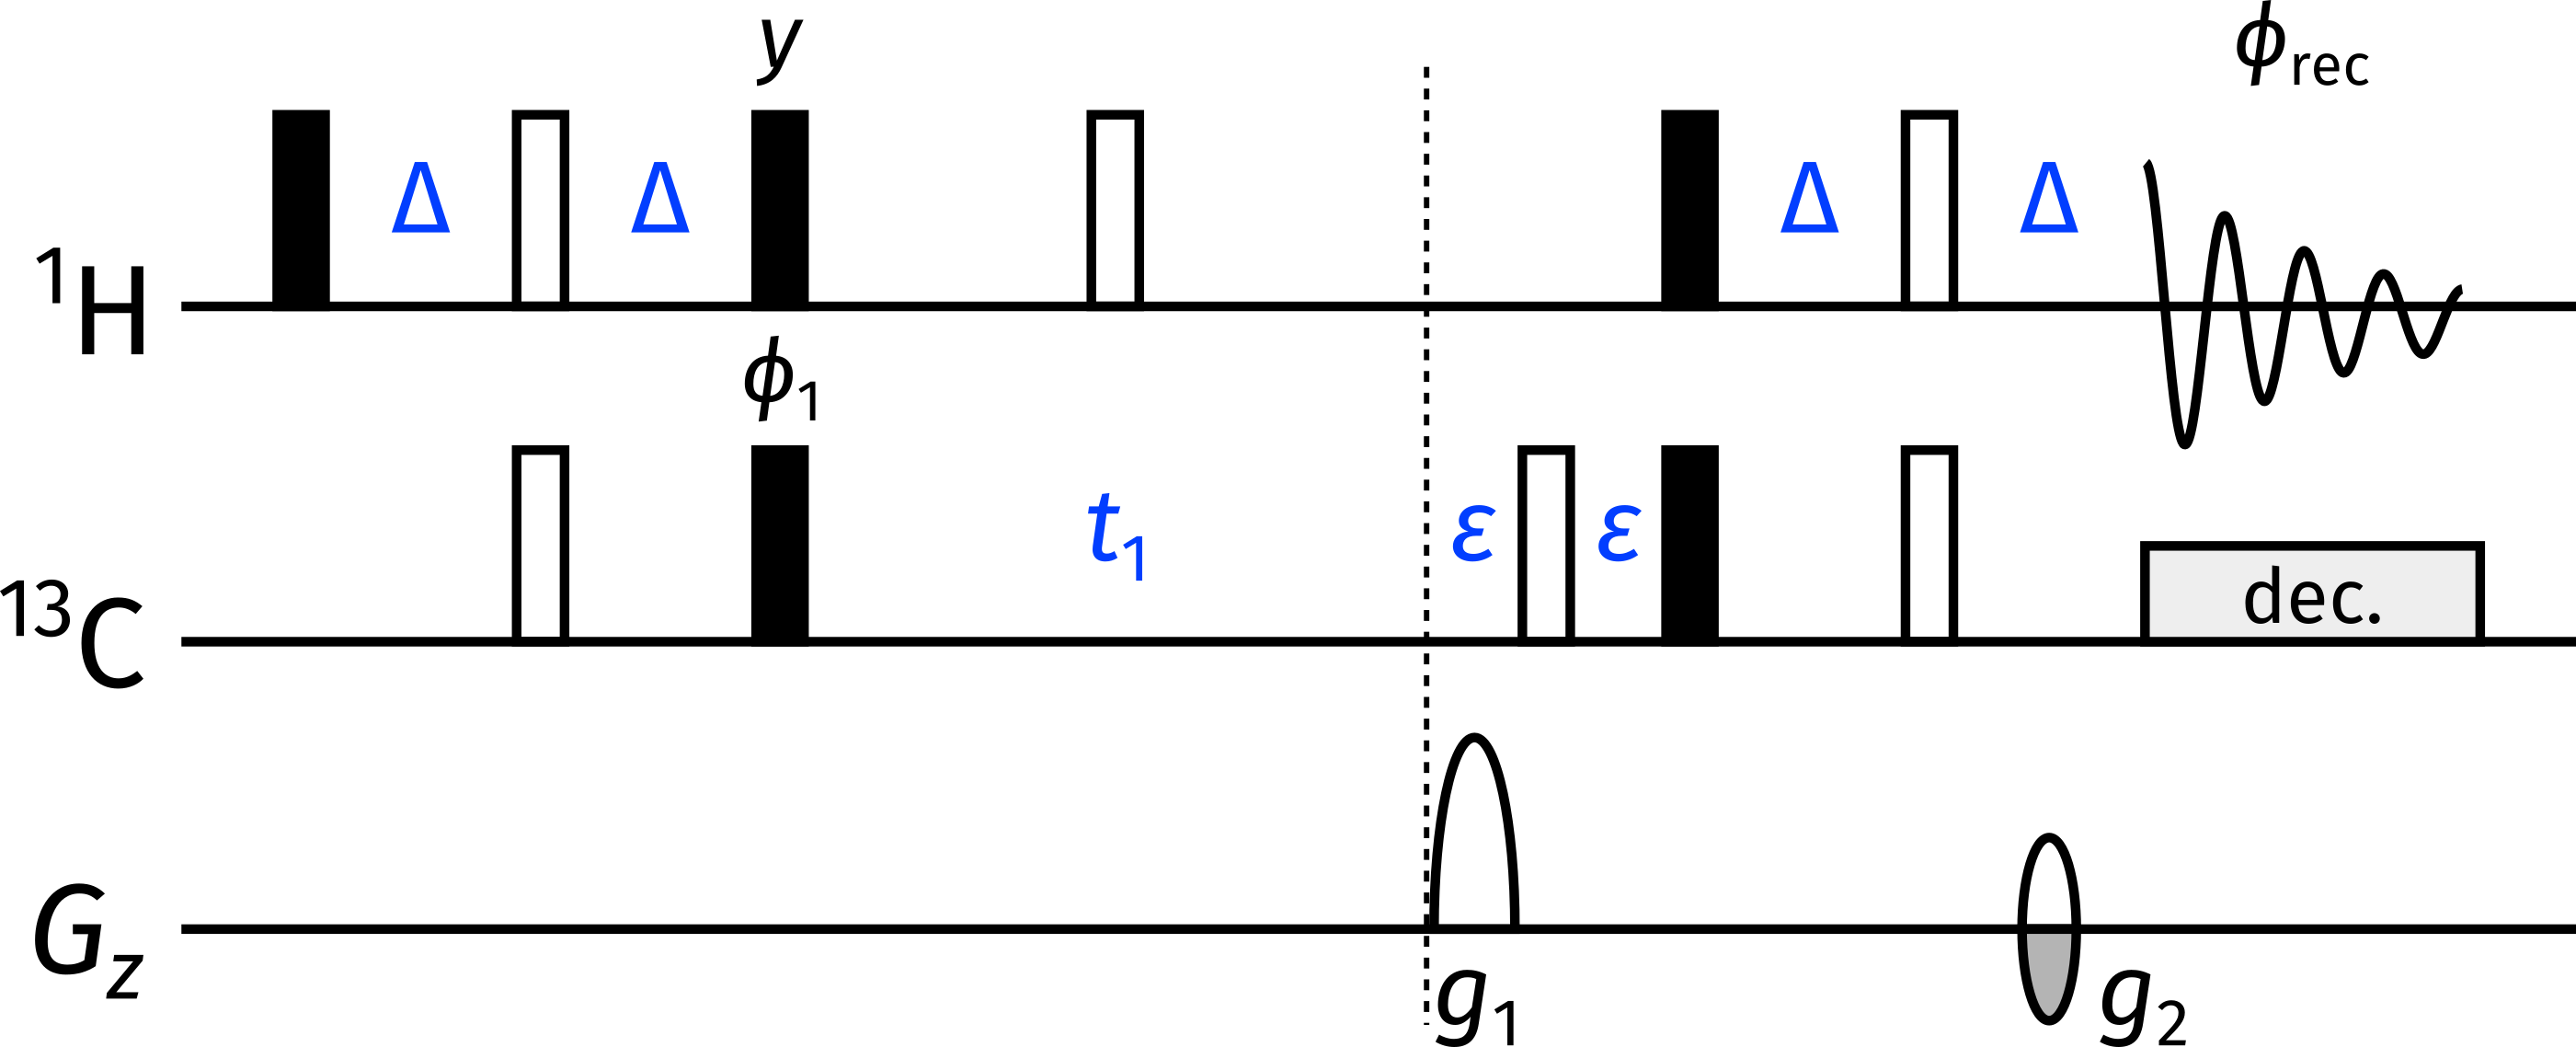
\includegraphics[scale=1.2]{pp/hsqc/hsqc_1grad.png}
    \caption[Echo--antiecho HSQC pulse sequence]{
        A typical echo--antiecho HSQC pulse sequence (the symbols are explained in the \textit{Preface}).
        The pulse phase $\phi_1$ and the receiver phase $\phi_\text{rec}$ are together alternated between $0$ and $\pi$; this is typically denoted as $\phi_1 = \phi_\text{rec} = (x, -x)$ as these phases correspond to the $+x$- and $-x$-axes.
        The delay $\Delta$ is set to $1/(4 \cdot \oneJ{CH})$.
        The gradient amplitudes are chosen such that $|g_1/g_2| = \gamma_{\ch{H}}/\gamma_{\ch{C}} \approx 4$.
        Echo--antiecho CTP selection is carried out by inverting the sign of $g_2$.
    }
    \label{fig:hsqc_1grad}
\end{figure}

The HSQC experiment seeks to only detect protons directly bonded to \carbon{}; all other protons must be suppressed.
We first show how pulsed field gradients and phase cycling allow the \textit{desired} signal to be obtained.

\todo{
This is technically only appropriate for an isolated methine (i.e. \ch{CH}) group.
The analysis which proceeds, however, is identical for methylene and methyl groups, which would be $I_2S$ and $I_3S$ systems respectively.
More unsound is the complete neglect of \ch{H}--\ch{H} coupling.
Luckily, this does not pose a serious problem here: it essentially leads to a small loss of signal.
However, for other experiments it may be necessary to account for $\nJ{HH}$: for example, it causes artefacts in the sensitivity-enhanced HSQC, as will be discussed in \cref{subsec:noah__sehsqc}.
In general, this illustrates the point that one should choose the \textit{simplest possible system} (but not one any simpler) to analyse a pulse sequence.
}


\todo{
\begin{itemize}
    \item CTP selection through gradients, mathematical requirement for CTP to be refocused
    \item Quadrature detection in $F_1$ (ugh)
    \item Composite coherence order\autocite{John1991JMR,Mitschang1995JCP}
    \item phase cycling to cancellation of unwanted peaks (e.g.\ arising from \ch{^{12}C}-bound \ch{^{1}H})
    \item explain why phase cycling (on its own) isn't really used for CTP selection any more
\end{itemize}
}




\printbibliography[heading=subbibnumbered]{}
